% ****** Start of file apssamp.tex ******
%
%   This file is part of the APS files in the REVTeX 4.2 distribution.
%   Version 4.2a of REVTeX, December 2014
%
%   Copyright (c) 2014 The American Physical Society.
%
%   See the REVTeX 4 README file for restrictions and more information.
%
% TeX'ing this file requires that you have AMS-LaTeX 2.0 installed
% as well as the rest of the prerequisites for REVTeX 4.2
%
% See the REVTeX 4 README file
% It also requires running BibTeX. The commands are as follows:
%
%  1)  latex apssamp.tex
%  2)  bibtex apssamp
%  3)  latex apssamp.tex
%  4)  latex apssamp.tex
%
\documentclass[%
reprint,
%linenumbers,
%superscriptaddress,
%groupedaddress,
%unsortedaddress,
%runinaddress,
%frontmatterverbose, 
%preprint,
%preprintnumbers,
%nofootinbib,
%nobibnotes,
%bibnotes,
 amsmath,amssymb,
 aps,
pra,
%prb,
%rmp,
%prstab,
%prstper,
floatfix,
showkeys
]{revtex4-2}

\usepackage{graphicx}% Include figure files
\usepackage{dcolumn}% Align table columns on decimal point
\usepackage{bm}% bold math
%\usepackage{hyperref}% add hypertext capabilities
%\usepackage[mathlines]{lineno}% Enable numbering of text and display math
%\linenumbers\relax % Commence numbering lines
%\usepackage[showframe,%Uncomment any one of the following lines to test 
%%scale=0.7, marginratio={1:1, 2:3}, ignoreall,% default settings
%%text={7in,10in},centering,
%%margin=1.5in,
%%total={6.5in,8.75in}, top=1.2in, left=0.9in, includefoot,
%%height=10in,a5paper,hmargin={3cm,0.8in},
%]{geometry}
\bibliographystyle{apsrev4-2}

\usepackage{mathtools}
\usepackage{tikz}
\usetikzlibrary{decorations.pathreplacing,calc}
\usetikzlibrary{arrows.meta}
\usetikzlibrary{calc,patterns,angles,quotes}

\usepackage{tabularx}  % For adjustable column widths
\usepackage{booktabs}  % For professional-quality table rules (\toprule, \midrule, etc.)
\usepackage{longtable}
\usepackage{hyperref}
%\usepackage{showlabels}
\usepackage{placeins}

\newtheorem{theorem}{Theorem}

\usepackage{xparse}
\NewDocumentCommand{\diff}{mg}{%
  \IfNoValueTF{#2}
    {\mathrm{d}#1}%
    {\frac{\mathrm{d}#1}{\mathrm{d}#2}}%
}

\usepackage{amsthm}
\usepackage[cal=boondox]{mathalfa}
%\usepackage{dutchcal}
% Macros for clarity
\begin{document}

\preprint{APS/123-QED}

\title{
On a Geometric Origin of Quantum Mechanics from Expanded Relativity
}% Force line breaks with \\
%\thanks{A footnote to the article title}%
\author{J. Manuel Oliveira \\ Email \href{mailto:j.m.oliveira.academic@outlook.com}{j.m.oliveira.academic@outlook.com}}
\affiliation{%
 Clinica Girassol\\
 Avenida Comandante Gika, 225\\
 Luanda\\
 Angola\\
}%
\date{\today}% It is always \today, today,
             %  but any date may be explicitly specified



\begin{abstract}
We develop a framework based on maximal spatiotemporal symmetry in which time is promoted to an on-shell three-dimensional vector subspace. Beginning from a general basis-independent $p$-temporal plus $q$-spatial linear transformation, the Principle of Relativity together with vectorial time selects a Lorentzian invariant for physically admissible transformations in the full $(p+q)$-dimensional spacetime. Compatibility of temporal-frame transport with this invariant fixes the direction of causal temporal translation, deriving the arrow of time from preservation of the relativistic interval and excluding the usual causal pathologies of multi-time theories. The temporal subspace nevertheless retains a residual rotation within the stabilizer of the causal direction. Relating this transverse rotation to four-dimensional translational action recovers the Planck--de Broglie relations, while its anti-Hermitian generator produces intrinsic spin and admits Abelian and non-Abelian field realizations. The associated angular-velocity relation yields a covariant field-transport equation containing a propagation-orthogonal geometric-source absent from the standard Dirac equation. In the geometric-source-free sector, the spinor realization recovers Dirac dynamics, and the quadratic reduction yields the Klein--Gordon mass shell and Pauli spin--field coupling. Admissible geometric-source structures generate mass, scalar Yukawa, charged-pion isospin, and anomalous magnetic-moment interactions. The resulting theory accommodates $\mathrm{U}(1)$, $\mathrm{SU}(2)$, and $\mathrm{SU}(3)$ sectors while preserving a positive-definite conserved density, four-dimensional relativistic kinematics, and Lorentzian causal propagation.
\end{abstract}


%\begin{description}
%\item[Usage]
%Secondary publications and information retrieval purposes.
%\item[Structure]
%You may use the \texttt{description} environment to structure your abstract;
%use the optional argument of the \verb+\item+ command to give the category of each item. 
%\end{description}


\keywords{
Vector time; Flag-and-Pole dynamics; Spatiotemporal symmetry; Clifford algebra; Quantum foundations; Relativistic wave equations
}%Use showkeys class option if keyword
                              %display desired
\maketitle

\tableofcontents


\section*{Latest version}\label{supmat_latest_version_note}
The most recent version of this manuscript is available at \url{https://joliverapps.github.io/ExpandedTheoryOfRelativity/}.



\section{Introduction}
\label{ch_intro}
Einstein's theory of relativity unifies space and time, yet it retains a structural asymmetry: space is a three-dimensional vector domain with intrinsic rotational freedom, whereas time enters as a one-dimensional direction. Expressing local displacements within their respective subspaces as $\mathbf{x}_{s}=x^{s}\mathbf{e}_{s}$ and $\mathbf{x}_{t}=x^{0}\mathbf{e}_{0}$ makes this asymmetry explicit and motivates the fundamental question: \emph{can time possess a three-dimensional vector structure without sacrificing the four-dimensional results of relativity or introducing the causal pathologies common to multi-time formulations; and, if so, how do the resulting dynamics connect to established physics?}

To address this question, we propose a framework built on the Principle of Relativity and the Principle of Maximal Spatiotemporal Symmetry. The latter posits that the temporal subspace possesses the same three-dimensional vector structure and algebraic status as the spatial subspace by default, unless physical consistency demands otherwise. From these premises, we demonstrate that the resulting framework is consistent and constitutes a single theory unifying special relativity and quantum physics.

Within this construction, temporal-frame compatibility with the relativistic invariant $c$ confines causal temporal displacement to a single stabilized temporal axis, thereby establishing a rigorous arrow of time. This constraint decomposes the six-dimensional spacetime into complementary $4+2$ sectors: a four-dimensional translational spacetime that exactly recovers Einsteinian relativity and an orthogonal two-dimensional temporal plane, termed the Plane-of-Now. The rotational structure of this Plane-of-Now gives rise to phase and spin degrees of freedom, Abelian and non-Abelian gauge structures, as well as mass, Yukawa, and isospin interactions, all without requiring additional independent postulates.

Thus, the Principle of Maximal Spatiotemporal Symmetry enlarges the underlying geometry without disturbing its established relativistic content. The resulting framework provides a common geometric foundation for the principal quantum and field-theoretic structures recovered by the theory while remaining exactly consistent with relativity and four-dimensional translational reality.

\subsection{Related Approaches in the Literature}
Endowing time with additional dimensions is not itself novel \cite{demers1975_vector_time,cole1980_particle_decay,kletetschka2025_three_dimensional_time}. Previous approaches employ temporal-orientation averaging \cite{cole1978_six_dimensional_relativity}, gauge constraints yielding one-time descriptions \cite{bars2000_2t_field_theory,bars_rey2001_sp2r_2t}, independent temporal variables and evolution parameters \cite{dirac1932_relativistic_qm,petrat_tumulka2014_multitime_qft,stueckelberg1941_temps_propre,horwitz_piron1973_relativistic_dynamics}, nonlocal constraints on initial data \cite{craig_weinstein2009_multiple_time}, or symmetry breaking that selects one observable time while leaving other temporal directions hidden \cite{DartoraCabrera2010}, while geometric interpretations of quantum phase have also been developed within four-dimensional spacetime \cite{hestenes2015_spacetime_algebra,hestenes1967_real_spinor_fields}.

The present theory does not use these mechanisms to restrict the temporal geometry. Instead, time remains a three-dimensional on-shell vector subspace with a structure symmetric to that of space. Compatibility with the relativistic invariant follows solely from the Principle of Relativity and the Principle of Maximal Spatiotemporal Symmetry, with equality between the six-dimensional velocity norm and its four-dimensional Lorentzian expression fixing the causal temporal direction. Accordingly, causal translation is confined to one temporal direction while the remaining two remain active as the Plane-of-Now, providing the geometric setting for quantum phenomena without additional causal clocks, compactification, gauge elimination of temporal components, hidden temporal directions, or supplementary geometric or dynamical constraints.

\subsection{Scope and Interpretation}
Before proceeding, two points must be clarified. First, the purpose of this foundational paper is to answer the question posed above and to establish the viability and internal coherence of the framework; it does not aim to exhaust every solution or experimental consequence. Second, this framework is an independent geometric theory, not a reformulation of standard quantum mechanics. No quantum structures or explicit relations to standard quantum mechanics are assumed a priori. The theory should therefore be evaluated strictly within its own postulates and internal consistency.

\subsection*{Notation and Conventions}
Bold calligraphic uppercase symbols denote six-dimensional vectors or full Clifford objects, such as $\boldsymbol{\mathcal{X}}$ and $\boldsymbol{\mathcal{Q}}$, while bold regular uppercase symbols denote four-dimensional vectors or Clifford operators in the translational sector, such as $\mathbf{U}$ and $\mathbf{G}$. Bold lowercase symbols denote objects restricted to a specified subspace, such as $\mathbf{x}_{s}$ and $\mathbf{x}_{t}$. Component notation follows a corresponding distinction: four-dimensional components are written with uppercase symbols and spacetime indices $\mu,\nu\in\{0,1,2,3\}$, as in $X^{\mu}$ and $P_{\mu}$; lowercase scalar components are retained for quantities defined within a specified spatial or temporal subspace, or used as scalar coordinates in the six-dimensional construction, as in $x^{s}$, $x^{t}$, and $x^{\alpha}$. Finally, the notation $O=\rho(\mathbf{O})$ identifies a chosen matrix representation of an abstract operator $\mathbf{O}$.


\section{Transformation of Coordinates}
\label{ch_Transformation_of_coordinates}
This section develops the coordinate transformation implied by the proposed spacetime geometry and establishes its relativistic content. The derivation clarifies the operational meaning of the Principle of Maximal Spatiotemporal Symmetry, verifies that vectorial time yields consistent and well-behaved relativistic kinematics, and shows that the usual Lorentz transformation arises as a special case of a general $(p+q)$-dimensional transformation obeying the Principle of Relativity.

\subsection{The Transformation Set}
To make the kinematic content concrete, consider two inertial observers $\mathrm{O}$ and $\mathrm{O}'$ whose relative motion induces both spatial and temporal vector displacements. Along their respective directions of motion, from the perspective of $\mathrm{O}$, the transformation takes the block form
\begin{subequations}
\begin{align}
    \mathbf{x}_{t} &= A(u,c)x'^{t}\mathbf{e}_{t} + B(u,c)x'^{s}\mathbf{e}_{t},\\
    \mathbf{x}_{s} &= C(u,c)x'^{t}\mathbf{e}_{s} + D(u,c)x'^{s}\mathbf{e}_{s},
\end{align}
\end{subequations}
where $u$ and $c$ represent the constant spatial and temporal displacement speeds associated with the inertial comparison, while $\mathbf{e}_{s}$ and $\mathbf{e}_{t}$ are the corresponding spatial and temporal unit directions. The kinematic coefficients $A, B, C, D \in \mathbb{R}$ depend exclusively on these constant relative speeds. Accordingly, the relative spatial and temporal displacement magnitudes measured by the two observers, from their own point of view, are written in parallel form as
\begin{equation}
    x^{s} = ut,\quad x^{t} = ct,\quad x'^{s} = ut',\quad x'^{t} = ct',
\end{equation}
so that the spatial and temporal sectors enter the kinematic construction on equal footing.

It is worth noticing that this block form does not describe a restricted $(1+1)$ model, but \emph{a homogeneous linear coordinate transformation valid in an arbitrary $(p+q)$-dimensional spacetime, with $p,q\in\mathbb{N}^{+}$ and a common origin}. Expanding the displacement direction vectors in a particular coordinate basis,
\begin{subequations}
\begin{align}
    \mathbf{e}_{t} &= \sum_{k=1}^{p}\hat{t}^{k}\mathbf{e}_{k},\quad \sum_{k=1}^{p}(\hat{t}^{k})^{2} = 1,\\
    \mathbf{e}_{s} &= \sum_{n=1}^{q}\hat{x}^{n}\mathbf{e}_{n},\quad \sum_{n=1}^{q}(\hat{x}^{n})^{2} = 1,
\end{align}
\end{subequations}
simply distributes the scalar coefficients componentwise into a system of $(p+q)$ equations of the same form, with $A^{k} = A\hat{t}^{k}$, $B^{k} = B\hat{t}^{k}$, $C^{n} = C\hat{x}^{n}$, and $D^{n} = D\hat{x}^{n}$, while leaving the scalar displacement magnitudes $x^{s}$ and $x^{t}$ unchanged.

Inertia requires the spatial and temporal direction vectors to be orthogonal; otherwise, objects initially at rest in the spatial subspace would not remain so as time progresses. Orthogonal vectors anticommute, so
\begin{equation}
    \mathbf{e}_{t}\mathbf{e}_{s} = -\mathbf{e}_{s}\mathbf{e}_{t}.
\end{equation}
For this initial kinematic construction, we choose the temporal unit-vector normalization
\begin{equation}
    \mathbf{e}_{t}^{2} = +1,
\end{equation}
which fixes the sign convention used to represent the temporal sector and is equivalent to a choice of metric signature. The spatial norm remains undetermined at this stage, leaving open whether the full spacetime is Euclidean or Lorentzian, so the spatial norm can take either value:
\begin{equation}
    \mathbf{e}_{s}^{2} = \varsigma, \quad \varsigma = +1 \quad \text{or} \quad \varsigma = -1.
\end{equation}

\subsection{The Scalar Relations}
Introduce the block-diagonal geometric operator
\begin{equation}
    \boldsymbol{\mathcal{Q}} =
    \begin{bmatrix}
        \mathbf{e}_{t} & 0\\
        0 & \mathbf{e}_{s}
    \end{bmatrix},
\end{equation}
together with the forward and inverse geometric boost matrices
\begin{subequations}\label{eq_boost_matrices}
\begin{align}
\boldsymbol{\mathcal{M}} &=
\begin{bmatrix}
    A\mathbf{e}_{t} & B\mathbf{e}_{t}\\
    C\mathbf{e}_{s} & D\mathbf{e}_{s}
\end{bmatrix},\\
\boldsymbol{\mathcal{M}}' &=
\begin{bmatrix}
    A\mathbf{e}_{t} & G\mathbf{e}_{t}\\
    H\mathbf{e}_{s} & D\mathbf{e}_{s}
\end{bmatrix}.
\end{align}
\end{subequations}
With $V = [x^{t},x^{s}]^{\mathrm{T}}$ and $V' = [x'^{t},x'^{s}]^{\mathrm{T}}$ collecting their respective scalar temporal and spatial displacement magnitudes, the direct and inverse transformations become
\begin{equation}
    V = \boldsymbol{\mathcal{Q}}^{-1}\boldsymbol{\mathcal{M}}V',\quad V' = \boldsymbol{\mathcal{Q}}^{-1}\boldsymbol{\mathcal{M}}'V.
\end{equation}
The Principle of Relativity requires the transformation to be invertible. Hence, the composition of the forward and inverse transformations yields the identity map,
\begin{equation}
    \boldsymbol{\mathcal{Q}}^{-1}\boldsymbol{\mathcal{M}}
    \boldsymbol{\mathcal{Q}}^{-1}\boldsymbol{\mathcal{M}}' = I,
\end{equation}
which leads to the scalar constraints
\begin{subequations}\label{eq_composition_constraints}
\begin{align}
    G &= -B,\\
    H &= -C,\\
    A &= D,\label{eq_AeqD}\\
    A^{2} - BC &= 1.
\end{align}
\end{subequations}

\subsection{Invariance of the Spacetime Norm}
Define the $(p+q)$-position vector in $\mathrm{O}$ by
\begin{equation}\label{eq_pq_position_def}
    \boldsymbol{\mathcal{X}} \coloneqq \mathbf{x}_{t} + \mathbf{x}_{s},\quad
    \mathbf{x}_{t} = x^{t}\mathbf{e}_{t},\quad
    \mathbf{x}_{s} = x^{s}\mathbf{e}_{s},
\end{equation}
so that applying the direct transformation together with $A = D$ gives
\begin{equation}
    \boldsymbol{\mathcal{X}}
    = \left(Ax'^{t} + Bx'^{s}\right)\mathbf{e}_{t}
    + \left(Cx'^{t} + Ax'^{s}\right)\mathbf{e}_{s},
\end{equation}
whose square produces the real quadratic form
\begin{equation}\label{eq_expansion_direct}
\begin{split}
    \boldsymbol{\mathcal{X}}^{2}
    &= (x^{t})^{2} + \varsigma(x^{s})^{2}= (A^{2}+ \varsigma C^{2})(x'^{t})^{2}\\
    &+ (B^{2}+ \varsigma A^{2})(x'^{s})^{2}
    + 2A(B + \varsigma C)x'^{t}x'^{s}.
\end{split}
\end{equation}
The inverse transformation likewise gives
\begin{equation}\label{eq_expansion_inverse}
\begin{split}
    \boldsymbol{\mathcal{X}}'^{2}
    &= (x'^{t})^{2} + \varsigma(x'^{s})^{2}= (A^{2} + \varsigma C^{2})(x^{t})^{2}\\
    &+ (B^{2} + \varsigma A^{2})(x^{s})^{2}
    - 2A(B + \varsigma C)x^{t}x^{s}.
\end{split}
\end{equation}
Since $\boldsymbol{\mathcal{X}}^{2}$ and $\boldsymbol{\mathcal{X}}'^{2}$ are real scalar norms of the same displacement, reciprocity and isotropy under the Principle of Relativity require
\begin{equation}
    \boldsymbol{\mathcal{X}}^{2} = \boldsymbol{\mathcal{X}}'^{2},
\end{equation}
so equating the coefficients yields
\begin{subequations}\label{eq_scalar_invariance_constraints}
\begin{align}
    A^{2} + \varsigma C^{2} &= 1,\\
    B^{2} + \varsigma A^{2} &= \varsigma,\label{eq_scalar_invariant_for_B}\\
    B + \varsigma C &= 0.
\end{align}
\end{subequations}
For $\varsigma = +1$, we have $B = -C$, and Eq.~\eqref{eq_scalar_invariant_for_B} reduces to
\begin{equation}
    A^{2} + B^{2} = 1,
\end{equation}
which confines the transformation to the circular trigonometric parameterization
\begin{equation}
    A(\varphi) = \cos\varphi,\quad B(\varphi) = \sin\varphi.
\end{equation}
For $\varsigma = -1$, by contrast, $B = C$, and Eq.~\eqref{eq_scalar_invariant_for_B} yields
\begin{equation}
    A^{2} - B^{2} = 1,
\end{equation}
with the hyperbolic parameterization
\begin{equation}
    A(\phi) = \cosh\phi \ge 1,\quad B(\phi) = \sinh\phi.
\end{equation}
Once the spatial and temporal axis directions have been selected, the pure inertial comparisons considered here vary only the relative translational motion, preserving those selections under successive collinear comparisons. However, as the unrestricted parameter $\varphi$ ranges over $\mathbb{R}$, the circular solution carries $A=D$ through positive, zero, and negative values. For $A<0$, successive ticks of a clock at rest in one frame receive decreasing time coordinates in the other, while the signed spatial separation of rod endpoints likewise reverses at the other frame's simultaneity\cite{Data2022_RevisitLorentzTransform}, introducing axis reversals into a comparison intended to describe relative motion alone.

Restricting the circular family to $A>0$ also fails to preserve closure under composition. Indeed, two transformations with $\varphi=\pi/3$ each have $A>0$, whereas their composition has parameter $2\pi/3$ and $A=-1/2$, so two valid changes of inertial frame would together produce an invalid. In contrast, the hyperbolic family preserves $A=D=\cosh\phi\ge1$ throughout $\phi\in\mathbb{R}$ and under arbitrary composition of collinear boosts. Thus, physical admissibility uniquely selects $\varsigma=-1$.

Under this signature, the invariant in a $(p+q)$-dimensional spacetime takes the form
\begin{equation}\label{eq_lorentz_interval}
    \boldsymbol{\mathcal{X}}^{2} = (x^{t})^{2} - (x^{s})^{2},
\end{equation}
which for $p=1$ and $q=3$ is the standard four-dimensional Lorentzian interval $\mathbf{X}^{2}$. In the maximally symmetric case $p=q=3$, the temporal component $\mathbf{x}_{t}$ can rotate while retaining its magnitude $x^{t}$, leaving the interval unchanged. Thus, at fixed $x^{t}$ and $x^{s}$, quantities obtained solely from this quadratic interval are independent of the choice of $p$ and $q$, while that choice determines the directions available to $\boldsymbol{\mathcal{X}}$ in the underlying linear space.

\subsection{The Invariant Limiting Speed}
Tracking the spatial origin of $\mathrm{O}'$ as described in $\mathrm{O}$ identifies the usual scalar relativistic parameters
\begin{equation}
    A = D = \gamma,\quad B = C = \beta\gamma,\quad \beta = \frac{u}{c},
\end{equation}
where $\gamma = (1 - \beta^{2})^{-1/2}$ is the Lorentz factor, so the boost in the selected temporal--spatial plane of a $p$-temporal plus $q$-spatial spacetime becomes
\begin{equation}\label{eq_extended_lorentz_transform}
    \begin{bmatrix}\mathbf{x}_{t}\\\mathbf{x}_{s}\end{bmatrix}
    = \gamma
    \begin{bmatrix}
        \mathbf{e}_{t} & \beta\mathbf{e}_{t}\\
        \beta\mathbf{e}_{s} & \mathbf{e}_{s}
    \end{bmatrix}
    \begin{bmatrix}x'^{t}\\x'^{s}\end{bmatrix}.
\end{equation}
Accordingly, the temporal and spatial vector transformations share the Lorentzian algebraic form, while $\mathbf{e}_{t}$ remains an a priori dynamical direction within the temporal subspace. Because $\beta = u/c$, real and finite boosts require $|u| < c$, identifying $c$ with the invariant limiting speed and, experimentally, with the speed of light in vacuum.

Because the spacetime norm is invariant, and the speed of light is universal in any $(p+q)$-dimensional spacetime obeying relativity, the usual definition of proper time,
\begin{equation}
\label{eq_pqvector_squared}
    \boldsymbol{\mathcal{X}}^{2}=\boldsymbol{\mathcal{X}} \cdot \boldsymbol{\mathcal{X}} = c^{2}\tau^{2},
\end{equation}
extends to these spaces, allowing for a generalized $(p+q)$-dimensional velocity defined as
\begin{equation}
    \boldsymbol{\mathcal{U}} \coloneqq \frac{\mathrm{d}\boldsymbol{\mathcal{X}}}{\mathrm{d}\tau},
\end{equation}
with norm $|\boldsymbol{\mathcal{U}}| = c$.

To establish this result, we first define a vector $\boldsymbol{\mathcal{V}}$ norm as
\begin{equation}
    |\boldsymbol{\mathcal{V}}| \coloneqq \sqrt{\boldsymbol{\mathcal{V}}^{2}},
\end{equation}
and differentiate $|\boldsymbol{\mathcal{X}}|^{2} = \boldsymbol{\mathcal{X}}^{2}$ for the position vector $\boldsymbol{\mathcal{X}}$ with respect to $\tau$ using the product rule on the inner product $\boldsymbol{\mathcal{X}}^{2} = \boldsymbol{\mathcal{X}} \cdot \boldsymbol{\mathcal{X}}$, which yields the kinematic relation
\begin{equation}
    \frac{\mathrm{d}}{\mathrm{d}\tau}|\boldsymbol{\mathcal{X}}| = \frac{\boldsymbol{\mathcal{X}} \cdot \boldsymbol{\mathcal{U}}}{|\boldsymbol{\mathcal{X}}|}.
\end{equation}
Substituting $|\boldsymbol{\mathcal{X}}| = c\tau$ back into this expression yields $\boldsymbol{\mathcal{X}} \cdot \boldsymbol{\mathcal{U}} = c |\boldsymbol{\mathcal{X}}| = c^{2}\tau$, which, for a homogeneous inertial trajectory that passes through the origin, gives $\boldsymbol{\mathcal{X}} = \tau \boldsymbol{\mathcal{U}}$, yielding
\begin{equation}\label{eq_squared_pqvelocity_norm}
    \boldsymbol{\mathcal{U}}^{2} = c^{2} \implies |\boldsymbol{\mathcal{U}}| = c.
\end{equation}
Because inertial frames are related by uniform motion, their reference trajectories are straight lines, so along a homogeneous inertial trajectory the finite interval relation in Eq.~\eqref{eq_pqvector_squared} gives the local differential form $(\mathrm{d}\boldsymbol{\mathcal{X}})^{2}=\mathrm{d}\boldsymbol{\mathcal{X}}\cdot\mathrm{d}\boldsymbol{\mathcal{X}}=c^{2}(\mathrm{d}\tau)^{2}$. Moreover, an accelerating observer in flat spacetime has an instantaneously comoving inertial frame at each event, so the local covariant relations established in inertial frames extend pointwise to smoothly accelerated observers. This extension, termed here the \emph{comoving inertial frames corollary}, will be used repeatedly throughout this paper, particularly in the derivation of the compatibility condition and the Planck--de Broglie relations.


\section{Recovering Einsteinian Special Relativity}
Pursuant to the principle of maximal spatiotemporal symmetry, from this section onward we specialize to a $p=3, q=3$ dimensional spacetime, recovering Einsteinian special relativity through the compatibility of spacetime norms.

\subsection{Classical Causal Time}
In the rest frame $\mathrm{O}$, the temporal displacement takes the form
\begin{equation}\label{eq_temporal_displacement_vector}
    \mathbf{x}_{t} \coloneqq x^{n}\mathbf{e}_{n}, \quad x^{n} = ct^{n}, \quad n \in \{4,5,6\},
\end{equation}
anchored by fixed, mutually orthogonal temporal basis vectors satisfying $\mathbf{e}_{n}^{2} = +1$.

Selecting a fiducial unit vector $\mathbf{e}_{0}$ to mark the temporal orientation at a reference event $\tau_{0}$, we introduce the rotor
\begin{equation}
    \boldsymbol{\omega}_{t} = \exp(-\mathbf{i}(\tau)\theta^{t}(\tau)), \quad \mathbf{i}^{\dagger} = -\mathbf{i}, \quad \mathbf{i}^{2} = -1,
\end{equation}
where $\mathbf{i}$ denotes a smooth unit temporal bivector and $\theta^{t}$ signifies a real angle parametrized such that $\theta^{t}(\tau_{0}) = 0$, yielding $\boldsymbol{\omega}_{t}(\tau_{0}) = 1$. Its transformation determines the evolved unit vector
\begin{equation}\label{eq_pole_from_flag}
    \mathbf{e}_{t} = \boldsymbol{\omega}_{t}\mathbf{e}_{0}\boldsymbol{\omega}_{t}^{\dagger},
\end{equation}
which establishes the radial displacement
\begin{equation}
    \mathbf{x}_{t} = c r^{t}\mathbf{e}_{t}, \quad r^{t} = \sqrt{(t^{4})^{2} + (t^{5})^{2} + (t^{6})^{2}}.
\end{equation}
Comparing this relation against the expression $\mathbf{x}_{t} = x^{t}\mathbf{e}_{t} = ct\mathbf{e}_{t}$, previously employed for temporal translations, directly equates the magnitude $r^{t}$ with classical time $t$.

Upon introducing the unit volume element of the temporal subspace,
\begin{equation}
    \mathbf{I}_{t} = \mathbf{e}_{4}\mathbf{e}_{5}\mathbf{e}_{6},
\end{equation}
the rotational bivector can subsequently be formulated in terms of a real unit vector $\mathbf{n}_{t}(\tau)$ orthogonal to the plane of rotation generated by the rotor,
\begin{equation}
    \mathbf{i} = \mathbf{I}_{t}\mathbf{n}_{t}.
\end{equation}
Within a specified temporal basis, the causal vector possesses direction cosines
\begin{equation}
    \mathbf{e}_{0} = \hat{\vartheta}^{k}\mathbf{e}_{k}, \quad \hat{\vartheta}^{k} \coloneqq \frac{t^{k}}{t}, \quad \sum_{k=4}^{6}(\hat{\vartheta}^{k})^{2} = 1,
\end{equation}
corresponding to the generator
\begin{equation}
    \mathbf{i} = \mathbf{e}_{5}\mathbf{e}_{6}\hat{\vartheta}^{4} + \mathbf{e}_{6}\mathbf{e}_{4}\hat{\vartheta}^{5} + \mathbf{e}_{4}\mathbf{e}_{5}\hat{\vartheta}^{6}.
\end{equation}
At this juncture, $\mathbf{n}_{t}$ remains free to fluctuate along arbitrary direction cosines bounded only by $t = \sqrt{(t^{4})^{2} + (t^{5})^{2} + (t^{6})^{2}}$. Nevertheless, as demonstrated below, the invariant norm of the spacetime velocity fixes the causal temporal direction, leaving the residual rotation confined to a static plane possessing $\mathbf{e}_{0}$ as its normal.

\subsection{The Fixed Causal Time Direction}
Previously, we established that $\boldsymbol{\mathcal{U}}^{2}=\left(\mathrm{d}\boldsymbol{\mathcal{X}}/\mathrm{d}\tau\right)^{2}=c^{2}$. To determine the directional consequences of this invariant, we return to the linear six-position defined in Eq.~\eqref{eq_pq_position_def} and decompose the spatial displacement across its static basis,
\begin{equation}
    \boldsymbol{\mathcal{X}}=\mathbf{x}_{t}+\mathbf{x}_{s}=ct\mathbf{e}_{t}+x^{a}\mathbf{e}_{a},\quad a\in\{1,2,3\},
\end{equation}
which, using $\mathrm{d}t/\mathrm{d}\tau=\gamma$ alongside $\mathrm{d}x^{a}/\mathrm{d}t=u^{a}$ and denoting $\mathrm{d}/\mathrm{d}\tau$ by an overdot, gives
\begin{equation}\label{eq_six_velocity}
    \boldsymbol{\mathcal{U}}=\frac{\mathrm{d}\boldsymbol{\mathcal{X}}}{\mathrm{d}\tau}=\gamma(c\mathbf{e}_{t}+u^{a}\mathbf{e}_{a})+ct\dot{\mathbf{e}}_{t}.
\end{equation}
Since the temporal and spatial sectors are mutually orthogonal, with $\mathbf{e}_{t}^{2}=+1$ and $\mathbf{e}_{a}^{2}=-1$, while differentiation of the temporal unit norm gives $\mathbf{e}_{t}\cdot\dot{\mathbf{e}}_{t}=0$, squaring the six-velocity yields
\begin{equation}
    \boldsymbol{\mathcal{U}}^{2}=\gamma^{2}(c^{2}-u^{2})+c^{2}t^{2}\dot{\mathbf{e}}_{t}^{2}=c^{2},
\end{equation}
where the initial term already recovers the Lorentzian invariant $\gamma^{2}(c^{2}-u^{2})=c^{2}$.

Because the origin of $t$ is arbitrary and $\boldsymbol{\mathcal{U}}^{2}=c^{2}$ holds for all $t$, the remaining contribution vanishes identically, giving
\begin{equation}
    \dot{\mathbf{e}}_{t}^{2}=0,
\end{equation}
which, since $\dot{\mathbf{e}}_{t}$ lies within the positive-definite temporal subspace, implies
\begin{equation}\label{eq_compatibility_condition}
    \dot{\mathbf{e}}_{t}=0.
\end{equation}
Although this fixed orientation is expected in inertial frames, the comoving inertial frames corollary extends the result locally to accelerated observers, so the causal temporal direction remains fixed along the accelerated worldline.

\subsection{Four-Dimensional Spacetime}
\label{ch_causality_preservation}
Rather than immutably locking the temporal subspace, this compatibility requirement restricts relative temporal rotations strictly to the plane governed by $\mathbf{e}_{0}$ as its stationary normal. Consequently,
\begin{equation}\label{eq_pon_normal_fixed}
    \mathbf{n}_{t}\equiv\mathbf{e}_{0},\quad \mathbf{i}=\mathbf{I}_{t}\mathbf{e}_{0} \implies \hat{\vartheta}^{k} =\mathrm{constant}.
\end{equation}
Due to the constancy of these coefficients, each distinct temporal coordinate simplifies to
\begin{equation}
    t^{k}=\hat{\vartheta}^{k}t,
\end{equation}
and as a result, the three temporal coordinates collapse to a functional dependence on a single scalar $t$, even though the underlying temporal manifold remains inherently three-dimensional.

The emerging $(4+2)$-dimensional structure consists of a translational manifold spanned by $\mathbf{e}_{0}$ and $\mathbf{e}_{a}$, characterized by the four-position
\begin{equation}
    \mathbf{X}=\mathbf{e}_{\mu}X^{\mu}(\tau),\quad \mu\in\{0,1,2,3\},\quad X^{0}=ct(\tau),
\end{equation}
alongside a temporal plane orthogonal to $\mathbf{e}_{0}$, whose residual rotational motion is driven by $\mathbf{i}$ and parametrized by $\theta^{t}(\tau)$. This subspace, designated as the \emph{Plane-of-Now}, accommodates a continuous spectrum of frame orientations at a given causal time $t$, thereby extending the point-like notion of ``now'' in conventional Einsteinian kinematics.

Across the translational sector, the basis vectors obey the standard Minkowski Clifford algebra
\begin{equation}\label{eq_minkowski_metric}
    \mathbf{e}_{\mu}\mathbf{e}_{\nu}+\mathbf{e}_{\nu}\mathbf{e}_{\mu}=2\eta_{\mu\nu}^{\mathrm{4D}},\quad \eta_{\mu\nu}^{\mathrm{4D}}=\mathrm{diag}(+1,-1,-1,-1),
\end{equation}
and both, the four-position and its corresponding proper-time derivatives reproduce standard special-relativistic kinematics—with $\mathbf{e}_{0}$ fixing the primary light-cone orientation—while the Plane-of-Now furnishes the internal rotational dynamics foundational to the quantum-mechanical constructs addressed below.

Adopting a basis that sets $\mathbf{e}_{0} = \mathbf{e}_{4}$, the direction cosines simplify to
\begin{equation}
    \hat{\vartheta}^{4} = 1, \quad \hat{\vartheta}^{5} = 0, \quad \hat{\vartheta}^{6} = 0,
\end{equation}
with the Plane-of-Now spanned by $\{\mathbf{e}_{5}, \mathbf{e}_{6}\}$ and generated by $\mathbf{i} = \mathbf{e}_{5}\mathbf{e}_{6}$. Owing to its algebraic simplicity, this adapted frame will serve as the primary reference for explicit representations.

\subsection{Visualization of the Six-Dimensional Spacetime as a Flag-and-Pole System}
\label{ch_flag_pole_visualization}

\begin{figure}[htbp]
\centering

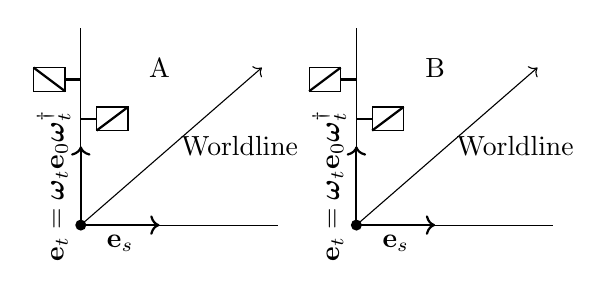
\begin{tikzpicture}
 % Define key coordinates A
 \coordinate (OriginA) at (0,0);
 \coordinate (TopYA) at (0,2.5);
 \coordinate (RighXA) at (2.5,0);
 \coordinate (StartWLA) at (0,0);
 \coordinate (EndWLA) at (2.3,2);

 % Flag 1 tips (Detached by 0.2, width 0.4)
 \coordinate (Flag1BottomLeft) at (0.2,1.2);
 \coordinate (Flag1BottomRight) at (0.6,1.2);
 \coordinate (Flag1TopLeft) at (0.2,1.5);
 \coordinate (Flag1TopRight) at (0.6,1.5);
 \coordinate (Arm1Pole) at (0,1.35);
 \coordinate (Arm1Flag) at (0.2,1.35);

 % Flag 2 tips
 \coordinate (Flag2BottomLeft) at (-0.2,1.7);
 \coordinate (Flag2BottomRight) at (-0.6,1.7);
 \coordinate (Flag2TopLeft) at (-0.2,2.0);
 \coordinate (Flag2TopRight) at (-0.6,2.0);
 \coordinate (Arm2Pole) at (0,1.85);
 \coordinate (Arm2Flag) at (-0.2,1.85);

 % Define key coordinates B
 \coordinate (OriginB) at (3.5,0);
 \coordinate (TopYB) at (3.5,2.5);
 \coordinate (RighXB) at (6.0,0);
 \coordinate (StartWLB) at (3.5,0);
 \coordinate (EndWLB) at (5.8,2);

 % Flag 3 tips
 \coordinate (Flag3BottomLeft) at (3.7,1.2);
 \coordinate (Flag3BottomRight) at (4.1,1.2);
 \coordinate (Flag3TopLeft) at (3.7,1.5);
 \coordinate (Flag3TopRight) at (4.1,1.5);
 \coordinate (Arm3Pole) at (3.5,1.35);
 \coordinate (Arm3Flag) at (3.7,1.35);

% Flag 4 tips
 \coordinate (Flag4BottomLeft) at (3.3,1.7);
 \coordinate (Flag4BottomRight) at (2.9,1.7);
 \coordinate (Flag4TopLeft) at (3.3,2.0);
 \coordinate (Flag4TopRight) at (2.9,2.0);
 \coordinate (Arm4Pole) at (3.5,1.85);
 \coordinate (Arm4Flag) at (3.3,1.85);
 
 % Draw the coordinate system A
 \fill (OriginA) circle (2pt) node[below left] {};
 \draw (OriginA) -- (RighXA);
 \draw (OriginA) -- (TopYA);
 \draw[thick, ->] (OriginA) -- ++(1,0) node[midway, below] {$\mathbf{e}_s$};
 \draw[thick, ->] (OriginA) -- ++(0,1) node[midway, left, rotate=90, anchor=south] {$\mathbf{e}_{t}=\boldsymbol{\omega}_{t}\mathbf{e}_{0}\boldsymbol{\omega}_{t}^{\dagger}$};
 
 % Draw Arm and Flag 1 (Scalar Base)
 \draw[thick] (Arm1Pole) -- (Arm1Flag);
 \draw (Flag1BottomRight) -- (Flag1BottomLeft) -- (Flag1TopLeft) -- (Flag1TopRight) -- cycle;
 \draw[thick] (Flag1BottomLeft) -- (Flag1TopRight);
 
 % Draw Arm and Flag 2 (Scalar Evolved - No Rotation)
 \draw[thick] (Arm2Pole) -- (Arm2Flag);
 \draw (Flag2BottomRight) -- (Flag2BottomLeft) -- (Flag2TopLeft) -- (Flag2TopRight) -- cycle;
 \draw[thick] (Flag2BottomLeft) -- (Flag2TopRight);
 
 % Draw worldline A
 \draw [->] (StartWLA) -- (EndWLA) node[midway, right] {Worldline};
 % Add an identification tag to diagram A
 \node at (1,2) {A};

 % Draw the coordinate system B
 \fill (OriginB) circle (2pt) node[below left] {};
 \draw (OriginB) -- (RighXB);
 \draw (OriginB) -- (TopYB);
 \draw[thick, ->] (OriginB) -- ++(1,0) node[midway, below] {$\mathbf{e}_s$};
 \draw[thick, ->] (OriginB) -- ++(0,1) node[midway, left, rotate=90, anchor=south] {$\mathbf{e}_{t}=\boldsymbol{\omega}_{t}\mathbf{e}_{0}\boldsymbol{\omega}_{t}^{\dagger}$};
 
 % Draw Arm and Flag 3 (Spinor Base)
 \draw[thick] (Arm3Pole) -- (Arm3Flag);
 \draw (Flag3BottomRight) -- (Flag3BottomLeft) -- (Flag3TopLeft) -- (Flag3TopRight) -- cycle;
 \draw[thick] (Flag3BottomLeft) -- (Flag3TopRight);
 
 % Draw Arm and Flag 4 (Spinor Twisted - 360 deg rotation)
 \draw[thick] (Arm4Pole) -- (Arm4Flag);
 \draw (Flag4BottomRight) -- (Flag4BottomLeft) -- (Flag4TopLeft) -- (Flag4TopRight) -- cycle;
 \draw[thick] (Flag4BottomRight) -- (Flag4TopLeft);


 % Draw worldline B
 \draw [->] (StartWLB) -- (EndWLB) node[midway, right] {Worldline};
 % Add an identification tag to diagram B
 \node at (4.5,2) {B};

\end{tikzpicture}

\caption{Flag-and-Pole depiction of the geometric framework. The stationary Pole direction $\mathbf{e}_{0}$ specifies the causal temporal axis and, in conjunction with the spatial frame (visualized as the ground), constitutes the Pole--ground coordinate system for the four-dimensional translational domain. The attached Flag embodies the temporal rotor $\boldsymbol{\omega}_{t}=\exp(-\mathbf{i}\theta^{t})$, whose operation produces the temporal vector $\mathbf{e}_{t}=\boldsymbol{\omega}_{t}\mathbf{e}_{0}\boldsymbol{\omega}_{t}^{\dagger}$. The angle $\theta^{t}$ parametrizes the angular movement of the Flag, whereas the generator $\mathbf{i}$ dictates its intrinsic algebraic rotation plane. Panels A and B depict alternative Flag configurations evaluated at identical proper time, highlighting how distinct rotational states map onto identical Pole--ground observables.}
\label{fig-FlagAndPoleDiag}
\end{figure}

With the causal temporal orientation locked via compatibility, Eq.~\eqref{eq_pole_from_flag} provides a vivid geometric representation of the temporal-frame architecture. In particular, the temporal space defined by $\mathbf{e}_{t}=\boldsymbol{\omega}_{t}\mathbf{e}_{0}\boldsymbol{\omega}_{t}^{\dagger}$, incorporating the rotor $\boldsymbol{\omega}_{t}=\exp(-\mathbf{i}\theta^{t})$, behaves precisely like a Flag-and-Pole system: the rigid Pole along $\mathbf{e}_{0}$ sets the causal temporal axis, whereas the attached Flag captures the action of the temporal rotor $\boldsymbol{\omega}_{t}$. Varying the orientation of the Flag through the parameter $\theta^{t}$ modulates the temporal rotational state without disturbing the underlying Pole--ground interval, while the generator $\mathbf{i}$—interpreted visually as an intrinsic twist within the Flag—governs the algebraic character of this rotation.



\section{Field Structure}
\subsection{Operational Consequences of the Compatibility Condition}
Expressing the compatibility condition explicitly yields
\begin{equation}\label{eq_compatibility_explicit}
    \dot{\mathbf{e}}_{t}=\dot{\boldsymbol{\omega}}_{t}\mathbf{e}_{0}\boldsymbol{\omega}_{t}^{\dagger}+\boldsymbol{\omega}_{t}\mathbf{e}_{0}\dot{\boldsymbol{\omega}}_{t}^{\dagger}=0,
\end{equation}
while differentiating the unitarity relation $\boldsymbol{\omega}_{t}^{\dagger}\boldsymbol{\omega}_{t}=1$ gives
\begin{equation}
    \dot{\boldsymbol{\omega}}_{t}^{\dagger}=-\boldsymbol{\omega}_{t}^{\dagger}\dot{\boldsymbol{\omega}}_{t}\boldsymbol{\omega}_{t}^{\dagger},
\end{equation}
so substitution into Eq.~\eqref{eq_compatibility_explicit} leads to
\begin{equation}
    \dot{\mathbf{e}}_{t}=\boldsymbol{\omega}_{t}\left[\boldsymbol{\omega}_{t}^{\dagger}\dot{\boldsymbol{\omega}}_{t},\mathbf{e}_{0}\right]\boldsymbol{\omega}_{t}^{\dagger}=0,
\end{equation}
which, owing to rotor invertibility, requires
\begin{equation}\label{eq_initial_commutator}
    \left[\boldsymbol{\omega}_{t}^{\dagger}\dot{\boldsymbol{\omega}}_{t},\mathbf{e}_{0}\right]=0.
\end{equation}
Within the three-dimensional temporal subspace, the bivectors commuting with $\mathbf{e}_{0}$ are proportional to $\mathbf{i}=\mathbf{I}_{t}\mathbf{e}_{0}$, so the compatible angular velocity lies in the plane orthogonal to the fixed causal direction. Since $\mathbf{I}_{t}$ and $\mathbf{e}_{0}$ are fixed in the common reference frame, Eq.~\eqref{eq_pon_normal_fixed} consequently gives $\dot{\mathbf{i}}=0$.

Furthermore, differentiating $\boldsymbol{\omega}_{t}=\cos\theta^{t}-\mathbf{i}\sin\theta^{t}$ for a unit temporal bivector satisfying $\mathbf{i}^{2}=-1$ and right-multiplying by $\boldsymbol{\omega}_{t}^{\dagger}$ yields
\begin{equation}
\begin{split}
    \dot{\boldsymbol{\omega}}_{t}\boldsymbol{\omega}_{t}^{\dagger}={}-\dot{\theta}^{t}\mathbf{i}-\frac{1}{2}\sin(2\theta^{t})\dot{\mathbf{i}}+\sin^{2}\theta^{t}\mathbf{i}\dot{\mathbf{i}},
\end{split}
\end{equation}
where the established constancy of $\mathbf{i}$ eliminates its derivative terms and leaves
\begin{equation}\label{eq_temporal_rotor_evolution}
    \dot{\boldsymbol{\omega}}_{t}\boldsymbol{\omega}_{t}^{\dagger}=\boldsymbol{\omega}_{t}^{\dagger}\dot{\boldsymbol{\omega}}_{t}=-\dot{\theta}^{t}\mathbf{i}.
\end{equation}
Consolidating Eqs.~\eqref{eq_pon_normal_fixed}, \eqref{eq_initial_commutator}, and \eqref{eq_temporal_rotor_evolution}, the compatibility requirement gives three primary operational relations,
\begin{subequations}\label{eq_spinor_compatibility_relations}
\begin{align}
    \dot{\mathbf{i}}=0\implies\dot{\hat{\vartheta}}^{k}&=0,\label{eq_temporal_generator_constancy}\\
    [\mathbf{i},\mathbf{e}_{0}]&=0,\label{eq_temporal_generator_commutator}\\
    [\boldsymbol{\omega}_{t}^{\dagger},\dot{\boldsymbol{\omega}}_{t}]&=0,\\
    \dot{\boldsymbol{\omega}}_{t}+\mathbf{i}\dot{\theta}^{t}\boldsymbol{\omega}_{t}&=0,\label{eq_temporal_rotor_transport}
\end{align}
\end{subequations}
where the first relation expresses constancy along the worldline through $\dot{\hat{\vartheta}}^{k}=U^{\mu}\partial_{\mu}\hat{\vartheta}^{k}$. In the common reference frame, the fixed temporal basis and its direction cosines provide the reference for the field realizations developed below.

\subsection{General Form of the Field}
The temporal rotation is characterized by the scalar angle $\theta^{t}$, its generator, and its composition law, independently of the specific geometric object being transformed. The vector-level action $\mathbf{e}_{t}=\boldsymbol{\omega}_{t}\mathbf{e}_{0}\boldsymbol{\omega}_{t}^{\dagger}$ with $\boldsymbol{\omega}_{t}=\exp(-\mathbf{i}\theta^{t})$ represents one concrete realization of this algebraic symmetry, whose action on other fields follows through their corresponding representations.

Consider an admissible field of type $F$ carrying a unitary representation of the compatible rotor subgroup. Letting $\boldsymbol{\Psi}_{F0}$ denote a fixed reference state and $\mathbf{i}_{F}$ the corresponding constant anti-Hermitian generator, the field along its temporal-rotation orbit is expressed as
\begin{equation}\label{eq_generalized_psi}
    \boldsymbol{\Psi}_{F}=\boldsymbol{\omega}_{tF}\boldsymbol{\Psi}_{F0},\quad \boldsymbol{\omega}_{tF}=\exp(-\mathbf{i}_{F}\theta^{t}),\quad \mathbf{i}_{F}^{\dagger}=-\mathbf{i}_{F},
\end{equation}
with composition and inverse relations
\begin{equation}
\begin{gathered}
    \boldsymbol{\omega}_{tF}(\theta_{1}^{t})\boldsymbol{\omega}_{tF}(\theta_{2}^{t})=\boldsymbol{\omega}_{tF}(\theta_{1}^{t}+\theta_{2}^{t}),\\
    \boldsymbol{\omega}_{tF}^{\dagger}=\boldsymbol{\omega}_{tF}^{-1}.
\end{gathered}
\end{equation}
Single-valued representations of this rotor subgroup inherit its parameter period and therefore satisfy
\begin{equation}
    \exp(-2\pi\mathbf{i}_{F})=1,
\end{equation}
while the transport relation in Eq.~\eqref{eq_temporal_rotor_transport} becomes
\begin{equation}\label{eq_starting_rotor_evolution}
    \dot{\boldsymbol{\omega}}_{tF}+\mathbf{i}_{F}\dot{\theta}^{t}\boldsymbol{\omega}_{tF}=0.
\end{equation}
The fixed reference element thus sweeps out its rotation orbit. In the real vector realization, the same rotation acts by the adjoint transformation
\begin{equation}
\begin{gathered}
    \boldsymbol{\omega}_{t}^{\mathrm{SO}(3)}\mathbf{v}\coloneqq\boldsymbol{\omega}_{t}\mathbf{v}\boldsymbol{\omega}_{t}^{\dagger},\\
    \mathbf{i}_{\mathrm{SO}(3)}\mathbf{v}\coloneqq\mathbf{i}\mathbf{v}-\mathbf{v}\mathbf{i},
\end{gathered}
\end{equation}
so the mappings
\begin{equation}
\begin{gathered}
    \boldsymbol{\Psi}_{F}\to\mathbf{e}_{t},\quad\boldsymbol{\Psi}_{F0}\to\mathbf{e}_{0},\\
    \boldsymbol{\omega}_{tF}\to\boldsymbol{\omega}_{t}^{\mathrm{SO}(3)},\quad\mathbf{i}_{F}\to\mathbf{i}_{\mathrm{SO}(3)}
\end{gathered}
\end{equation}
give $\mathbf{i}_{\mathrm{SO}(3)}\mathbf{e}_{0}=[\mathbf{i},\mathbf{e}_{0}]=0$. Consequently, this real rotation fixes the causal direction while rotating transverse temporal vectors through an angle $2\theta^{t}$ within the plane orthogonal to $\mathbf{e}_{0}$.

Within the common reference frame, the chosen generator satisfies
\begin{equation}
    \dot{\mathbf{i}}_{F}=0,
\end{equation}
while the field realization may admit a larger algebra $\mathfrak{g}_{F}$ containing additional generators. For nonzero $\mathbf{i}_{F}$, choosing a positive-definite inner product in which this generator has unit norm and an orthonormal basis $\{\mathbf{i}_{\beta}\}$ gives
\begin{equation}\label{eq_generator_direction}
\begin{gathered}
    \mathbf{i}_{F}=\hat{\vartheta}^{\beta}\mathbf{i}_{\beta},\quad\sum_{\beta=1}^{\dim\mathfrak{g}_{F}}(\hat{\vartheta}^{\beta})^{2}=1,\\
    \beta\in\{1,\ldots,\dim\mathfrak{g}_{F}\},
\end{gathered}
\end{equation}
where $\hat{\vartheta}^{\beta}$ specifies the generator direction within $\mathfrak{g}_{F}$ and $\theta^{t}$ retains the rotor-angle normalization inherited above. In the temporal vector realization, the three temporal bivectors are dual to their normal directions, so their coefficients correspond to the temporal direction cosines.

\subsubsection{Field Representation and Spin}
The Lie bracket closure
\begin{equation}
    [\mathbf{i}_{\beta},\mathbf{i}_{\gamma}]=f_{\beta\gamma}{}^{\delta}\mathbf{i}_{\delta}
\end{equation}
defines the structure of $\mathfrak{g}_{F}$. Selecting its associated group $G_{F}$ and a unitary representation
\begin{equation}
    \rho_{F}:G_{F}\rightarrow U(V_{F})
\end{equation}
determines the matrix generator
\begin{equation}
    \mathfrak{i}_{F}\coloneqq d\rho_{F}(\mathbf{i}_{F})\in d\rho_{F}(\mathfrak{g}_{F})\subseteq\mathfrak{u}(F),
\end{equation}
and hence the matrix rotor and field state,
\begin{equation}
\begin{gathered}
    w_{F}\coloneqq\rho_{F}(\boldsymbol{\omega}_{tF})=\exp(-\mathfrak{i}_{F}\theta^{t}),\\
    \Psi_{F}=w_{F}\Psi_{F0},
\end{gathered}
\end{equation}
where $V_{F}\cong\mathbb{C}^{F}$ and $\Psi_{F0},\Psi_{F}$ are the corresponding column states. Unitarity then gives $\Psi_{F}^{\dagger}\Psi_{F}=\Psi_{F0}^{\dagger}\Psi_{F0}$, with $\theta^{t}$ describing evolution along the chosen orbit.

Representative field spaces and their admitted algebras include
\begin{equation}
    (V_{F},\mathfrak{g}_{F})\in\bigl\{(\mathbb{C}^{1},\mathfrak{u}(1)),(\mathbb{C}^{2},\mathfrak{su}(2)),(\mathbb{C}^{3},\mathfrak{su}(3))\bigr\},
\end{equation}
where $F=\dim_{\mathbb{C}}V_{F}$ counts the complex field components. The scalar, spinor, and vector realizations are organized by this component count, expressed through the spin index $j$ as
\begin{equation}
    F=2j+1.
\end{equation}
Thus, the one-component scalar field carries the $U(1)$ phase action, the two-component spin-$\frac{1}{2}$ field carries the fundamental action of $SU(2)$, and the three-component spin-$1$ field carries the fundamental action of $SU(3)$. The phase generator $\mathfrak{i}_{F}$ describes the selected temporal rotation, while any additional admitted field transformations belong to the broader algebra.

For the three-component realization, the real rotation subgroup follows by restricting $SU(3)$ to transformations preserving $\mathbb{R}^{3}\subset\mathbb{C}^{3}$, giving
\begin{equation}
    SU(3)\cap GL(3,\mathbb{R})=SO(3),
\end{equation}
or, at the Lie-algebra level,
\begin{equation}
    \mathfrak{su}(3)\cap\mathfrak{gl}(3,\mathbb{R})=\mathfrak{so}(3).
\end{equation}
Accordingly, a real initial vector remains real under the corresponding generator,
\begin{equation}
    \mathfrak{i}_{F}\in\mathfrak{so}(3),\quad\Psi_{F0}\in\mathbb{R}^{3}\implies\Psi_{F}\in\mathbb{R}^{3},
\end{equation}
retaining three real components with the natural vector rotation action. The full $SU(3)$ realization acts on the complex three-component field, while its real $SO(3)$ subgroup supplies this vector realization. Spacetime dependence remains parameterized by $X^{\mu}$, with proper-time evolution evaluated along $X^{\mu}(\tau)$.

\subsubsection{Gauge Covariance and Non-Abelian Fields}\label{ch_gauge_covariance}
Because the phase origin of $\theta^{t}$ is arbitrary, the Principle of Relativity demands that field equations exhibit covariance under local shifts of this origin. Such a transformation acts on the temporal rotor according to
\begin{equation}
\begin{gathered}
    \boldsymbol{\omega}_{tF}'=\exp[-\mathbf{i}_{F}(\theta^{t}+\delta\theta^{t})]=\mathbf{g}\boldsymbol{\omega}_{tF},\\
    \mathbf{g}=\exp(-\mathbf{i}_{F}\delta\theta^{t}),
\end{gathered}
\end{equation}
where $\delta\theta^{t}(X)$ represents the local angular displacement, with $\delta\theta^{t}(\tau)=\delta\theta^{t}(X(\tau))$ along a trajectory.

Expanding $\mathbf{i}_{F}=\hat{\vartheta}^{\beta}\mathbf{i}_{\beta}$ in the admitted generator basis, the local transformation becomes
\begin{equation}
\begin{gathered}
    \mathbf{g}=\exp[-\alpha^{\beta}(X)\mathbf{i}_{\beta}],\\
    g_{F}\coloneqq\rho_{F}(\mathbf{g})=\exp[-\alpha^{\beta}(X)T_{\beta}],
\end{gathered}
\end{equation}
with
\begin{equation}
\begin{gathered}
    T_{\beta}\coloneqq d\rho_{F}(\mathbf{i}_{\beta}),\\
    \alpha^{\beta}(X)=\delta\theta^{t}(X)\hat{\vartheta}^{\beta}\in\mathbb{R}.
\end{gathered}
\end{equation}
These proportional parameters describe the selected phase orbit, while general reference changes within the admitted group use independent $\alpha^{\beta}(X)$. Under this action, the abstract field transforms in tandem with the temporal rotor,
\begin{equation}
\begin{gathered}
    \boldsymbol{\Psi}_{F}\mapsto\mathbf{g}\boldsymbol{\Psi}_{F},\quad w_{F}\mapsto g_{F}w_{F},\\
    \Psi_{F}\mapsto g_{F}\Psi_{F},
\end{gathered}
\end{equation}
so the same covariance applies to every subsequent equation containing derivatives of the temporal rotor. The Principle of Relativity therefore leads to the corresponding gauge-covariant derivative and, through its standard construction, the Abelian or non-Abelian potentials associated with the admitted $U(1)$, $SU(2)$, and $SU(3)$ field structures.


\section{Fundamentals of Flag Dynamics}\label{ch_EqOfMotion}
\subsection{Temporal-Frame Rotation and the Planck--de Broglie Relations}\label{ch_temporal_rotation_momentum}
Applying the chain rule to Eq.~\eqref{eq_starting_rotor_evolution} gives
\begin{equation}
    \frac{\mathrm{d}\boldsymbol{\omega}_{tF}}{\mathrm{d}\tau} = \frac{\mathrm{d}X^{\mu}}{\mathrm{d}\tau}\partial_{\mu}\boldsymbol{\omega}_{tF} = U^{\mu}\partial_{\mu}\boldsymbol{\omega}_{tF},\quad \frac{\mathrm{d}\theta^{t}}{\mathrm{d}\tau} = U^{\mu}\partial_{\mu}\theta^{t},
\end{equation}
and defining the local angular covector as
\begin{equation}
    K_{\mu} \coloneqq \partial_{\mu}\theta^{t},
\end{equation}
puts the temporal-frame evolution into the form
\begin{equation}\label{eq_parallel_transport}
    U^{\mu}\left(\partial_{\mu} + \mathbf{i}_{F}K_{\mu}\right)\boldsymbol{\omega}_{tF} = 0.
\end{equation}
The covector $K_{\mu}$ acts as the wave four-covector of the Flag-time roll, measuring the local rate of Plane-of-Now rotation along the four-dimensional transport path through
\begin{equation}\label{eq_flag_angle_differential}
    \mathrm{d}\theta^{t} = K_{\mu}\mathrm{d}X^{\mu}.
\end{equation}
The corresponding local Hamilton--Jacobi description is determined by the Hamilton principal function $S(X^{\mu})$, whose on-shell differential is
\begin{equation}\label{eq_action_differential}
    \mathrm{d}S = \partial_{\mu}S\mathrm{d}X^{\mu} = P_{\mu}\mathrm{d}X^{\mu},
\end{equation}
where
\begin{equation}\label{eq_def_canonical_momentum}
    P_{\mu} \coloneqq \partial_{\mu}S
\end{equation}
is the canonical momentum conjugate to displacement.

For a free inertial particle, both $P_{\mu}$ and $K_{\mu}$ are constant, so the corresponding scalar increments vary linearly along the same inertial trajectory and are therefore proportional to one another, giving $\Delta S=\xi\Delta\theta^{t}$ with constant $\xi$. Because these inertial relations are strictly linear, the proportionality remains valid in the infinitesimal limit, giving
\begin{equation}\label{eq_action_temporalangle_relation}
    \mathrm{d}S = \xi\mathrm{d}\theta^{t}.
\end{equation}
In the free rest configuration, both covectors are purely temporal, so this relation establishes the local correspondence
\begin{equation}\label{eq_momentum_wavevector}
    \partial_{\mu}S = \xi\partial_{\mu}\theta^{t} \implies P_{\mu} = \xi K_{\mu}.
\end{equation}
Since both quantities transform as four-covectors, this proportionality holds in every inertial frame and, again by the comoving inertial frames corollary, extends locally to any observer in flat spacetime. Decomposing them into their standard components,
\begin{equation}
    P_{\mu} = \left(\frac{E}{c}, -\mathbf{p}\right),\quad K_{\mu} = \left(\frac{\omega}{c}, -\mathbf{k}\right),
\end{equation}
gives
\begin{equation}
    E = \xi\omega,\quad \mathbf{p} = \xi\mathbf{k},
\end{equation}
so identification with the Planck--de Broglie relations fixes the empirical proportionality scale,
\begin{equation}
    \xi = \hbar.
\end{equation}
Writing the canonical four-momentum as
\begin{equation}
    P_{\mu} = mU_{\mu} + q_{\beta}A_{\mu}^{\beta},
\end{equation}
allows the gauge contribution to be incorporated into the gauge-covariant geometric derivative
\begin{equation}
    \boldsymbol{\nabla}_{\mu} \coloneqq \partial_{\mu} + \frac{\mathbf{i}_{F}}{\hbar}q_{\beta}A_{\mu}^{\beta},
\end{equation}
so substituting $K_{\mu} = P_{\mu}/\hbar$ into Eq.~\eqref{eq_parallel_transport} and using $U^{\mu}U_{\mu} = c^{2}$ yields the mass-scaled transport relation
\begin{equation}\label{eq_transport_mass}
    \left(U^{\mu}\boldsymbol{\nabla}_{\mu} + \mathbf{i}_{F}\frac{mc^{2}}{\hbar}\right)\boldsymbol{\omega}_{tF} = 0.
\end{equation}

\subsection{Clifford Form and the geometric-source}
In Eq.~\eqref{eq_transport_mass}, the four-velocity contracts with the derivative of the rotor field rather than acting algebraically on the field itself. Recasting the transport law into Clifford form allows the equation to be projected along the propagation direction, shifting this dependence into a direct algebraic action. Because the four-velocity possesses a fixed invariant norm, this algebraic action can be resolved via projectors onto its propagation eigenspaces, effectively eliminating the explicit four-velocity dependence. As a byproduct of this geometric reformulation, a propagation-orthogonal geometric-source (PO-Source) emerges that is absent in the standard Dirac equation.

For a spinor realization, take
\begin{equation}
    \mathbf{i}_{F} \to \mathbf{i}\in\mathfrak{su}(2),\quad \mathbf{i}^{2} = -1,\quad [\mathbf{i}, \mathbf{e}_{\mu}] = 0.
\end{equation}
Introducing the four-velocity vector and the Clifford covariant derivative,
\begin{equation}
    \mathbf{U} \coloneqq \mathbf{e}_{\mu}U^{\mu},\quad \mathbf{D}^{\flat} \coloneqq \mathbf{e}^{\mu}\boldsymbol{\nabla}_{\mu},\quad \mathbf{e}^{\mu} \coloneqq \eta_{\mathrm{4D}}^{\mu\nu}\mathbf{e}_{\nu},
\end{equation}
Eq.~\eqref{eq_transport_mass} can be recast into the geometric form
\begin{equation}\label{eq_transport_geometric}
    \mathbf{U}\cdot\left(\mathbf{i}\mathbf{D}^{\flat} - \frac{m}{\hbar}\mathbf{U}\right)\boldsymbol{\omega}_{t} = 0.
\end{equation}
Since Eq.~\eqref{eq_transport_geometric} constrains only the contraction along $\mathbf{U}$, the uncontracted Clifford expression need not vanish. Denoting this expression by the Clifford geometric-source $\mathbf{G}$ separates the transport law into the equivalent system
\begin{subequations}\label{eq_rotor_geometric_source_system}
    \begin{align}
        \left(\mathbf{i}\mathbf{D}^{\flat} - \frac{m}{\hbar}\mathbf{U}\right)\boldsymbol{\omega}_{t} &= \mathbf{G},\label{eq_source_field_def}\\
        \mathbf{U}\cdot\mathbf{G} &= 0.\label{eq_G_field_constraint}
    \end{align}
\end{subequations}
These relations define distinct solution problems. Eq.~\eqref{eq_G_field_constraint} determines the admissible PO-sources independently of the rotor equation, while Eq.~\eqref{eq_source_field_def} determines the rotor evolution for a specified $\mathbf{G}$. Every pair $(\boldsymbol{\omega}_{t}, \mathbf{G})$ satisfying this system thus solves Eq.~\eqref{eq_transport_geometric}. Conversely, every solution of Eq.~\eqref{eq_transport_geometric} generates such a pair through Eq.~\eqref{eq_source_field_def}.

The choice $\mathbf{G} = 0$ immediately satisfies Eq.~\eqref{eq_G_field_constraint} and defines the geometric-source-free sector, whose propagation projection recovers two decoupled Dirac equations for the particle and antiparticle sectors. Geometrically, the compatible rotor leaves a vector parallel to the causal Pole invariant while acting nontrivially on transverse structures.

Parameterizing the Clifford geometric-source by a left-acting Clifford operator $\mathbf{R}$,
\begin{equation}\label{eq_G_R_definition}
    \mathbf{G} \coloneqq \frac{1}{\hbar}\mathbf{R}\boldsymbol{\omega}_{t},
\end{equation}
gives the sourced Clifford rotor equation
\begin{equation}\label{eq_clifford_rotor}
    \left(\mathbf{i}\mathbf{D}^{\flat} - \frac{m}{\hbar}\mathbf{U} - \frac{1}{\hbar}\mathbf{R}\right)\boldsymbol{\omega}_{t} = 0,
\end{equation}
and, because the compatible rotor is even and satisfies $[\mathbf{U},\boldsymbol{\omega}_{t}]=0$, its invertibility reduces the propagation-orthogonality constraint to
\begin{equation}\label{eq_R_field_constraint}
    \left(\mathbf{U}\cdot\mathbf{R}\right)\boldsymbol{\omega}_{t} = 0 \implies \mathbf{U}\cdot\mathbf{R} = 0.
\end{equation}
The field-action reality condition derived from the Lagrangian formulation in Appendix~\ref{appx_spinor_lagrangian} further requires
\begin{equation}
    \mathbf{I}_{t}\mathbf{R}^{\dagger}\mathbf{I}_{t} = -\mathbf{R} \iff \mathbf{e}_{0}\mathbf{R}^{\dagger}\mathbf{e}_{0} = -\mathbf{i}\mathbf{R}\mathbf{i},
\end{equation}
which, for an operator preserving the Plane-of-Now sectors through $[\mathbf{i}, \mathbf{R}] = 0$, simplifies to
\begin{equation}
    \mathbf{e}_{0}\mathbf{R}^{\dagger}\mathbf{e}_{0} = \mathbf{R}.
\end{equation}
Under a local change of field frame, with the Clifford basis transported by conjugation,
\begin{equation}
    \boldsymbol{\omega}_{t}' = \mathbf{g}\boldsymbol{\omega}_{t},\quad \mathbf{i}' = \mathbf{g}\mathbf{i}\mathbf{g}^{-1},\quad \mathbf{R}' = \mathbf{g}\mathbf{R}\mathbf{g}^{-1},
\end{equation}
the geometric-source transforms covariantly,
\begin{equation}
    \mathbf{G}' = \frac{1}{\hbar}\mathbf{R}'\boldsymbol{\omega}_{t}' = \mathbf{g}\mathbf{G},
\end{equation}
while $\mathbf{U}'=\mathbf{g}\mathbf{U}\mathbf{g}^{-1}$ preserves the corresponding source constraint. Transformations preserving the selected generator satisfy $[\mathbf{g},\mathbf{i}]=0$, giving $\mathbf{i}'=\mathbf{i}$, and those preserving the propagation frame also satisfy $[\mathbf{g},\mathbf{U}]=0$.

\subsubsection{Removal of the Explicit Four-Velocity Dependence through Projection}
Introducing the matrix representations of the operators in Eq.~\eqref{eq_clifford_rotor},
\begin{equation}
    D^{\flat} \coloneqq \rho(\mathbf{D}^{\flat}),\quad U \coloneqq \rho(\mathbf{U}),\quad R \coloneqq \rho(\mathbf{R}),
\end{equation}
right-multiplication of its represented form by the fixed initial module element $\Psi_{0}$ converts the temporal-rotor evolution equation into an equation for the dynamically evolved module field $\Psi = w_{t}\Psi_{0}$,
\begin{equation}\label{eq_clifford_module}
    \mathfrak{i}D^{\flat}\Psi - \frac{m}{\hbar}U\Psi - \frac{1}{\hbar}R\Psi = 0.
\end{equation}
The algebraic action $U\Psi$ can then be resolved on the eigenspaces of the normalized propagation matrix
\begin{equation}
    \hat{\mathbf{U}}\coloneqq\frac{\mathbf{U}}{c}, \quad \hat{U} =\rho(\hat{\mathbf{U}})= \frac{U}{c},\quad \hat{U}^{2} = I,
\end{equation}
using the complementary projectors
\begin{equation}
    \Pi_{\pm} \coloneqq \frac{1}{2}\left(I \pm \hat{U}\right),\quad \Pi_{\pm}^{2} = \Pi_{\pm},\quad \Pi_{\pm}\Pi_{\mp} = 0.
\end{equation}
For a solution belonging to either propagation eigenspace,
\begin{equation}
    \Pi_{\pm}\Psi = \Psi \implies \hat{U}\Psi = \pm\Psi \implies U\Psi = \pm c\Psi,
\end{equation}
so, substitution into Eq.~\eqref{eq_clifford_module} using the short-hand notations
\begin{equation}
    \kappa \coloneqq \frac{mc}{\hbar}, \quad \chi \coloneqq \frac{1}{\hbar},
\end{equation}
replaces the algebraic four-velocity action by its eigenvalue and yields the generalized field equation
\begin{equation}\label{eq_clifford_field}
    \left(\mathfrak{i}D^{\flat} \mp \kappa I_{8} - \chi R\right)\Psi = 0.
\end{equation}

\subsection{The Spinor Field Equation and the Dirac Limit}
\label{ch_spinor_matrix_representation}
The spinor field equation follows directly from Eq.~\eqref{eq_clifford_field} by specifying an explicit matrix realization of $Cl(3,3)$. In the adapted temporal basis $\mathbf{e}_{4} = \mathbf{e}_{0}$, choose
\begin{equation}
    \rho(\mathbf{e}_{\mu}) = I_{2} \otimes \gamma_{\mu},\quad \mu \in \{0, 1, 2, 3\},
\end{equation}
for the four-dimensional translational sector and
\begin{equation}
    \rho(\mathbf{e}_{5}) = \sigma_{x} \otimes \gamma_{5},\quad \rho(\mathbf{e}_{6}) = \sigma_{y} \otimes \gamma_{5},
\end{equation}
for the Plane-of-Now basis vectors. The corresponding rotation generator is therefore
\begin{equation}
    \mathfrak{i} = \rho(\mathbf{e}_{5})\rho(\mathbf{e}_{6}) = i\Sigma_{z},\quad \Sigma_{z} \coloneqq \sigma_{z} \otimes I_{4}.
\end{equation}
In the same basis,
\begin{equation}
    \rho(\mathbf{e}^{\mu}) = \eta_{\mathrm{4D}}^{\mu\nu}\rho(\mathbf{e}_{\nu}) = I_{2} \otimes \gamma^{\mu},\quad \gamma^{\mu} \coloneqq \eta_{\mathrm{4D}}^{\mu\nu}\gamma_{\nu},
\end{equation}
so the mixed operator takes the form
\begin{equation}\label{eq_spinor_gamma_definition}
    \rho(\mathbf{i}\mathbf{e}^{\mu}) = i\Gamma^{\mu},\quad \Gamma^{\mu} \coloneqq \sigma_{z} \otimes \gamma^{\mu}.
\end{equation}
The gauge-covariant derivative is likewise represented block-diagonally as
\begin{equation}\label{eq_spinor_covariant_derivative}
    D_{\mu} \coloneqq \rho(\boldsymbol{\nabla}_{\mu}) = \begin{bmatrix}I_{4}D_{\mu}^{+} & 0 \\ 0 & I_{4}D_{\mu}^{-}\end{bmatrix},\quad \mathfrak{i}D^{\flat} = i\Gamma^{\mu}D_{\mu}
\end{equation}
with
\begin{equation}\label{eq_sector_covariant_derivatives}
    D_{\mu}^{\pm} = \partial_{\mu} \pm \frac{i}{\hbar}q_{\beta}A_{\mu}^{\beta}.
\end{equation}
Accordingly, the physical column field is built from two stacked Dirac spinors, while the represented geometric-source operator takes the corresponding block form,
\begin{equation}
    \Psi = \begin{bmatrix}\Psi_{+} \\ \Psi_{-}\end{bmatrix},\quad R = \begin{bmatrix}R_{++} & R_{+-} \\ R_{-+} & R_{--}\end{bmatrix},
\end{equation}
and Eq.~\eqref{eq_clifford_field} becomes
\begin{equation}\label{eq_fundamental_matrix}
    \left(i\Gamma^{\mu}D_{\mu} \mp \kappa I_{8} - \chi R\right)\Psi = 0.
\end{equation}
This system contains two Dirac spinors with conjugate gauge phases. For $R = 0$, the blocks decouple into particle and antiparticle sectors, with the lower block brought to the standard Dirac form by $\Psi_{-} \mapsto \gamma_{5}\Psi_{-}$. Their conjugate gauge couplings arise from the opposite temporal rotations generated by $\mathfrak{i} = i\Sigma_{z}$ and remain independent of the propagation branches $U\Psi = \pm c\Psi$, so both sectors coexist on the same future-directed branch.

A nonzero geometric-source $\mathbf{R}$ that commutes with the Plane-of-Now bivector, $[\mathbf{i},\mathbf{R}]=0$, preserves the two sectors and decouples this equation into two Dirac equations with extra terms from the geometric-source. Conversely, if this condition is not achieved, the two sectors become rigidly coupled, as in the case of an isospin interaction examined in the Lagrangian formulation in Appendix~\ref{appx_spinor_lagrangian}.

Finally, the geometric-algebra isomorphism
\begin{equation}
    Cl(3,3) \cong M_{8}(\mathbb{R})
\end{equation}
shows that the underlying Clifford algebra admits an eight-dimensional real matrix representation. In the complex basis used here, the reality of the corresponding spinor module is expressed by
\begin{equation}
    \Psi_{-}=\gamma_{5}C\bar{\Psi}_{+}^{\mathsf T},
\end{equation}
where $C$ is the charge-conjugation matrix. The Pauli and Dirac matrices therefore make the connection to conventional spinor equations transparent while retaining the real Clifford structure.

\subsection{Universal Second-Order Equation and Pauli Structure}
\label{ch_quadratic_pauli_structure}
For the future-directed propagation branch, define the mass-geometric-source operator
\begin{equation}
    M \coloneqq \kappa I_{8} + \chi R,
\end{equation}
so that acting on Eq.~\eqref{eq_clifford_field} with the complementary operator $\mathfrak{i}D^{\flat} + M$ and multiplying the resulting equation by $-1$ gives the second-order wave equation
\begin{equation}\label{eq_2order_full_source}
    \left(D^{\mu}D_{\mu} + \mathfrak{i}q \chi F + \left[\mathfrak{i}D^{\flat}, M\right] + M^{2}\right)\Psi = 0,
\end{equation}
where, for a gauge sector with nonzero coupling $q$, the represented gauge-covariant field-strength is
\begin{equation}\label{eq_general_field_strength_bivector}
    F \coloneqq \rho(\mathbf{F}),\quad \mathbf{F} \coloneqq -\frac{\mathbf{i}}{2q\chi}\mathbf{e}^{\mu}\mathbf{e}^{\nu}[\boldsymbol{\nabla}_{\mu}, \boldsymbol{\nabla}_{\nu}].
\end{equation}
For simultaneous gauge sectors, $qF$ denotes the sum $\sum_{r}q_{r}F^{(r)}$, with this definition applied separately to the covariant derivatives of each gauge sector $r$. The gauge-curvature term supplies the minimal Pauli interaction, while the commutator and quadratic terms generated by $R$ describe the differential and algebraic contributions of the geometric-source, opening an additional physical channel for nonminimal magnetic-moment corrections and their non-Abelian analogues.

Unlike the first-order equation, whose differential operator $D^{\flat} = \rho(\mathbf{e}^{\mu})D_{\mu}$ explicitly carries the represented translational Clifford basis and therefore constrains the field to a compatible module, the second-order equation has the representation-independent principal operator $D^{\mu}D_{\mu}$. It consequently admits realization on any admissible field space $V_{F} \cong \mathbb{C}^{F}$ with $\mathfrak{i} \in \mathfrak{u}(F)$ for which $qF$, $M$, and the commutator contribution act consistently on that space.

For $R = 0$, Eq.~\eqref{eq_2order_full_source} reduces to the standard quadratic Dirac--Pauli form,
\begin{equation}
    \left(D^{\mu}D_{\mu} + \mathfrak{i}q \chi F + \kappa^2 \right)\Psi = 0,
\end{equation}
whose $\mathfrak{su}(2)$ spinor realization yields the baseline expectation $g = 2$, while in the scalar realization of the same geometric-source-free sector,
\begin{equation}
    \mathfrak{i} \to i \in \mathfrak{u}(1),\quad \Psi \to \psi \in \mathbb{C},
\end{equation}
the bivector spin action is trivial, so the quadratic equation reduces to the Klein--Gordon equation
\begin{equation}
    \left(D^{\mu}D_{\mu} + \kappa^{2}\right)\psi = 0.
\end{equation}
Although introduced as shorthand notation, the mass-geometric-source composition operator $M = \kappa I_{8} + \chi R$ hints at a profound relationship between mass and solutions to the propagation-orthogonality problem. In Appendix~\ref{appx_spinor_lagrangian}, we show that this relationship is no coincidence: mass, the Yukawa interaction, the isospin interaction, and non-minimal field-strength solutions explaining anomalous moments can all be derived from a total PO-source satisfying $\mathbf{U}\cdot \mathbf{R}_{\mathrm{total}} = 0$ under the gauge-covariance and reality conditions given above.


\section{Results}
\subsection{Anomalous Propagation-Orthogonal Geometric-Sources}
In the adapted basis, using $U=\rho(\mathbf{U})$, $\hat{U}=U/c$, $R=\rho(\mathbf{R})$, $\mathfrak{i}=\rho(\mathbf{i})=i\Sigma_{z}$, and $X^{\ddagger}=\Gamma^{0}X^{\dagger}\Gamma^{0}$, we establish in Appendix~\ref{appx_general_matrix_source} that the general matrix solution to the propagation-orthogonality constraint for an even-grade element of the algebra takes the form $R_{\mathrm{e}}=\frac{1}{2}f(\tau)\left(A_{\mathrm{e}}+\hat{U}A_{\mathrm{e}}\hat{U}\right)$, subject to $[U,R_{\mathrm{e}}]=0$, where $A_{\mathrm{e}}\in M_{8}(\mathbb{C})$ is an even seed matrix satisfying $KA_{\mathrm{e}}K=A_{\mathrm{e}}$, with $K=\sigma_z\otimes\gamma_5$.

Writing $h_{\mu\nu}=-\frac{1}{q\chi}\mathfrak{i}\rho([\boldsymbol{\nabla}_{\mu},\boldsymbol{\nabla}_{\nu}])$, the gauge curvature $F=\rho(\mathbf{F})$ takes the matrix form
\begin{equation}
    F=\frac{1}{2}\left(I_{2}\otimes\gamma^{\mu}\gamma^{\nu}\right)h_{\mu\nu},\quad h_{\mu\nu}=-h_{\nu\mu}.
\end{equation}
For the electromagnetic Abelian field strength $F_{\mathrm{EM}}$, for which $h_{\mu\nu}$ has real coefficients, the seed
\begin{equation}
    A_{\mathrm{B}}=\mathfrak{i}F_{\mathrm{EM}}
\end{equation}
satisfies the even seed condition $KA_{\mathrm{B}}K=A_{\mathrm{B}}$, and the solution
\begin{equation}
    R_{\mathrm{B}}=\frac{1}{2}f(\tau)\left(A_{\mathrm{B}}+\hat{U}A_{\mathrm{B}}\hat{U}\right),\quad f(\tau)\in\mathbb{R},
\end{equation}
further satisfies
\begin{equation}
    R_{\mathrm{B}}^{\ddagger}=R_{\mathrm{B}},\quad [U,R_{\mathrm{B}}]=0,\quad [\mathfrak{i},R_{\mathrm{B}}]=0,
\end{equation}
while the electromagnetic gauge-transformation law ensures gauge covariance, fulfilling the requirements for an admissible PO-source.

The curvature projection isolates the magnetic bivector relative to $\hat{U}$,
\begin{equation}\label{eq_projected_magnetic_matrix}
    B=\frac{1}{2}\left(F_{\mathrm{EM}}+\hat{U}F_{\mathrm{EM}}\hat{U}\right) \implies R_{\mathrm{B}}=\mathfrak{i}f(\tau)B,
\end{equation}
retaining three independent spatial bivector components in the propagation rest frame, with the squared magnetic-field magnitude
\begin{equation}
    |B|^{2}\coloneqq-\frac{1}{8}\operatorname{tr}\left(B^{2}\right) \ge 0.
\end{equation}
Since $(\mathfrak{i}B)^2=|B|^2I_8$, choosing a real function $f(\tau)=qa(|B|^2)$ gives the magnetic anomalous-moment source
\begin{equation}\label{eq_nonlinear_magnetic_source}
    R_{\mathrm{B}}=\mathfrak{i}qa(|B|^2)B, \quad a(|B|^2)\in\mathbb{R},
\end{equation}
where $q$ is the electric charge of the matter field. With $B=\rho(\mathbf{B})$, the corresponding abstract source is
\begin{equation}
    \mathbf{R}_{\mathrm{B}}=\mathbf{i}qa\mathbf{B}, \quad R_{\mathrm{B}}=\rho(\mathbf{R}_{\mathrm{B}}),
\end{equation}
where the argument of $a$ is suppressed for brevity.

Because $\mathbf{i}$ and $\mathbf{B}$ are bivectors in mutually orthogonal subspaces, $\mathbf{R}_{\mathrm{B}}$ has grade four in the full Clifford algebra, while its simplest dependence on the electromagnetic field strength is linear. Its lowest-order nonlinear polynomial extension is
\begin{equation}\label{eq_cubic_magnetic_source}
    R_{\mathrm{B}}=\mathfrak{i}q\left(a_0+a_2|B|^2\right)B, \quad a_0,a_2\in\mathbb{R},
\end{equation}
where $a_0$ and $a_2$ are dimensional constants. The additional term is cubic in the magnetic field because $|B|^2\mathfrak{i}B=(\mathfrak{i}B)^3$. We take $a_0\neq0$ to retain the simplest nonzero linear interaction as the leading contribution; setting $a_2=0$ recovers that linear solution exactly.

\subsubsection{Weak-Field Pauli Interaction and Schwinger Limit}
For $a_{0}\neq0$, the ratio of the cubic to the linear contribution is $|a_{2}/a_{0}|\,|B|^2$, so the weak-field approximation gives
\begin{equation}
    R_{\mathrm{B}}\simeq \mathfrak{i}a_{0}qB,\quad |B|\ll\sqrt{\left|\frac{a_{0}}{a_{2}}\right|}.
\end{equation}
Sector preservation, together with the block-diagonal electromagnetic covariant derivative, allows Eq.~\eqref{eq_fundamental_matrix} to separate into particle and antiparticle sectors. For a configuration purely magnetic in the propagation rest frame, restriction to the positive Flag-time sector gives
\begin{equation}
    H_{B}\Psi_+=i\hbar\partial_t\Psi_+,
\end{equation}
with
\begin{equation}\label{eq_magnetic_test_hamiltonian}
    \begin{split}
        H_{B}={}&c\boldsymbol{\alpha}\cdot\left[-i\hbar\nabla-q\boldsymbol{A}\right]\\
        &+\beta mc^2+q\Phi I_4+iqa_{0}c\beta B,
    \end{split}
\end{equation}
where $\beta\coloneqq\gamma^0$, $\alpha^j\coloneqq\gamma^0\gamma^j$, and $B_j=(\nabla\times\boldsymbol{A})_j$; in this Hamiltonian, $B$ denotes its $4\times4$ positive-sector block. Comparison with the magnetic Dirac--Pauli interaction~\cite{pauli1941_relativistic} identifies the weak-field anomalous coupling as $a_{\mathrm{weak}}=2\kappa a_{0}$, so that
\begin{equation}
    a_{0}=\frac{a_{\mathrm{weak}}}{2\kappa}.
\end{equation}
For the electron, matching to Schwinger's leading QED result~\cite{schwinger1948_magnetic_moment} gives
\begin{equation}
    a_{\mathrm{0}}^{\mathrm{electron}}=\frac{\alpha}{4\pi\kappa_{\mathrm{electron}}},
\end{equation}
where $\alpha$ is the fine-structure constant.

\subsubsection{The Nonminimal Cubic Solution for Anomalous Response}
The cubic extension also has an established effective-field-theory counterpart. In the same purely magnetic sector, $F_{\alpha\beta}F^{\alpha\beta}=2|B|^2$ and $iB=\frac{1}{2}\sigma^{\mu\nu}F_{\mu\nu}$, where $\sigma^{\mu\nu}\coloneqq\frac{i}{2}[\gamma^\mu,\gamma^\nu]$. Defining
\begin{equation}
    O_5=\bar{\Psi}_+\sigma^{\mu\nu}\Psi_+F_{\mu\nu},\quad O_9=(F_{\alpha\beta}F^{\alpha\beta})O_5,
\end{equation}
the contribution of the PO-source becomes
\begin{equation}
    -\chi\bar{\Psi}_+R_+\Psi_+=-\frac{q\chi a_{0}}{2}O_5-\frac{q\chi a_{2}}{4}O_9,
\end{equation}
where $R_+$ is the positive Flag-time restriction of $R_{\mathrm{B}}$ and $\chi=1/\hbar$. These operators have canonical mass dimensions five and nine, respectively. The linear dipole operator appears in Eq.~(3.29) of Ref.~\cite{li2021_left_dim9}, while $O_9$ is a Hermitian combination of the cubic operators listed in Eqs.~(3.488) and (3.513) and their conjugates.

Thus, both the Pauli interaction and the cubic magnetic coupling featured in effective field theories arise directly within the algebraic solution space of propagation orthogonality. In standard QED, the Pauli structure appears through radiative corrections to the electromagnetic vertex, with Schwinger's leading contribution supplied by a finite one-loop Pauli form factor~\cite{schwinger1948_magnetic_moment}; the present framework yields the Pauli and cubic magnetic operator structures algebraically from propagation orthogonality.


\section{Discussion}
Extending time to a three-dimensional vector subspace allows the Flag-and-Pole framework to recover several foundational structures of relativity and quantum physics from a common temporal geometry. The admissible inertial branch has a pseudo-Euclidean realization with three positive temporal and three negative spatial directions, while the corresponding quadratic displacement norm reduces exactly to the Lorentzian interval. Temporal-frame compatibility then fixes a single causal temporal direction, eliminating the two possible tilt modes and confining temporal translation to the stabilized Pole-time axis. The transverse temporal directions nevertheless remain physically active through rotation within the Plane-of-Now, so the theory retains standard four-dimensional relativistic kinematics and causality without suppressing the underlying three-dimensional structure of time.

This geometric separation yields two scalar measures of evolution, with proper time $\tau$ parametrizing Pole--ground motion and the Flag-time angle $\theta^{t}$ measuring temporal rotation along the normalized direction $\mathbf{i}_{F}=\hat{\vartheta}^{\beta}\mathbf{i}_{\beta}$. Just as the Principle of Relativity requires covariance under changes of the proper-time reference, $\tau\mapsto\tau+\delta\tau$, the same requirement applied to the Flag-time reference, $\theta^{t}\mapsto\theta^{t}+\delta\theta^{t}$, yields gauge covariance. The general field construction accommodates unitary representations, and applying this covariance requirement to the established Abelian and non-Abelian structures naturally introduces the corresponding $U(1)$, $SU(2)$, and $SU(3)$ gauge potentials.

Beyond field representations, the connection between wave and particle descriptions follows from the fundamental relation $dS=\xi\,d\theta^{t}$, which identifies an infinitesimal change of classical action with the corresponding Flag-time rotation through a universal scale. With $P_{\mu}=\partial_{\mu}S$ and $K_{\mu}=\partial_{\mu}\theta^{t}$, this relation gives $P_{\mu}=\xi K_{\mu}$ in the free rest configuration and, by Lorentz covariance, in every inertial frame. The experimentally established Planck--de Broglie relations fix this universal scale as $\xi=\hbar$. Wave--particle complementarity therefore reflects the same free motion expressed through translational action and temporal rotation, with minimal coupling extending this relation to the gauge-covariant temporal-rotor transport law.

From this dynamical foundation, the theory identifies two distinct classes of sources, both of purely geometric origin. First, gauge-covariance geometric sources (GC-sources) arise because the Principle of Relativity requires equations containing derivatives of the temporal rotor to remain covariant under local transformations $g_{F}\in U(V_{F})$, thereby retaining the same form for all inertial observers in the full six-dimensional spacetime. Second, propagation-orthogonal geometric sources (PO-sources) arise algebraically from the rotor action itself rather than from the requirement of covariance of the dynamical equations: the rotor acts trivially on geometric components parallel to transport but remains nontrivial on components orthogonal to $\mathbf{U}$.

These two source mechanisms intersect when the gauge curvature associated with a GC-source possesses a propagation-orthogonal component. Projecting this curvature relative to $\mathbf{U}$ converts it into a PO-source, providing the geometric origin of anomalous-moment interactions. Because this source inherits both the gauge curvature and its propagation-dependent decomposition, its form may be more complex than the forms arising directly from the Plane-of-Now algebra, unless additional symmetry or dynamics ultimately reduces it to a simple closed-form expression.

Finally, although measurement probabilities are not developed here, the six-dimensional geometry suggests a possible basis for them. An observer restricted to the four-dimensional spacetime selected by the causal temporal direction cannot access the complete initial temporal state and can therefore specify it only through statistical inference, making the resulting uncertainty structurally epistemic rather than ontological. Once this initial description is assigned, the rotor, or its wave-function representation, tracks the subsequent evolution of all compatible possibilities. Apart from the hypothesis presented, the theory already yields the positive-definite density $J^{0} = \Psi^{\dagger}\Psi \ge 0$, permitting the usual probability-density interpretation of the wave function to be incorporated into the present framework as an experimental contingency rather than a derived result.


\section{Conclusions}
The central conclusion of this work is that treating time as a three-dimensional vector subspace remains compatible with established relativistic physics while providing a geometric origin for structures conventionally introduced as independent elements of quantum mechanics and quantum field theory. Within this architecture, the arrow of time, complex phase, intrinsic spin, wave--particle complementarity, gauge covariance, Abelian and non-Abelian gauge structures, mass, scalar Yukawa interactions, charged-pseudoscalar isospin exchange, and anomalous magnetic-moment interactions arise from distinct aspects of the same temporal geometry.

Taken together, these results answer the guiding question of this work affirmatively and thereby fulfill its stated scope. More broadly, they lay the foundations for a consistent theory of quantum physics in which Einsteinian relativity and quantum structures arise together from a common six-dimensional geometry, rather than quantum dynamics being independently postulated and subsequently constrained to conform to a pre-existing relativistic spacetime. This common origin distinguishes the present unification from existing approaches, while the framework's economy and broad results offer a promising route to general unification.


\appendix

\section{General Matrix Solution of the Propagation-Orthogonality Constraint}\label{appx_general_matrix_source}
In the adapted basis, let $U=\rho(\mathbf{U})$, $\hat{U}=U/c$, and $R=\rho(\mathbf{R})$, with $\mathbf{U}^{2}=c^{2}$ and $\mathfrak{i}=\rho(\mathbf{i})$. The PO-source conditions are
\begin{equation}\label{eq_source_admissibility}
    \mathbf{U}\cdot\mathbf{R}=0,\quad R^{\ddagger}=R,\quad R'=gRg^{-1},
\end{equation}
where $g=\rho(\mathbf{g})$ represents an admissible local field-frame transformation and
\begin{equation}
    X^{\ddagger}\coloneqq\Gamma^{0}X^{\dagger}\Gamma^{0}, \quad \Gamma^{0}=\sigma_z\otimes\gamma^{0}.
\end{equation}
For a homogeneous grade-$r$ component $\mathbf{R}_r$, the contraction is given by
\begin{equation}
    \mathbf{U}\cdot\mathbf{R}_r=\frac{1}{2}\left(\mathbf{U}\mathbf{R}_r-(-1)^r\mathbf{R}_r\mathbf{U}\right),
\end{equation}
which shows that propagation orthogonality requires commutation for even grades and anticommutation for odd grades. Because contraction lowers grade, these conditions hold separately for each component of an inhomogeneous PO-source, with the scalar component satisfying the constraint identically.

In the chosen matrix realization, grade involution is represented by
\begin{subequations}
    \begin{align}
        &X\mapsto KXK, \quad K=\sigma_z\otimes\gamma_5,\\
        &\{K,\hat{U}\}=0, \quad [K,\mathfrak{i}]=0.
    \end{align}
\end{subequations}
The represented constraint becomes
\begin{equation}\label{eq_matrix_source_constraint}
    \rho\!\left(\mathbf{U}\cdot\mathbf{R}\right)=\frac{1}{2}(UR-KRKU)=0,
\end{equation}
whose general solution, for an arbitrary seed matrix $A\in M_8(\mathbb{C})$, is
\begin{equation}\label{eq_general_matrix_source}
    R=P(A)\coloneqq\frac{1}{2}\left(A+\hat{U}KAK\hat{U}\right).
\end{equation}
Because the projection map is idempotent, $P(P(A))=P(A)$, the constraint is equivalent to $P(R)=R$. Consequently, every solution is obtained by choosing $A=R$, although any seed $A=R+N$ with $P(N)=0$ yields the same PO-source.

The projection also satisfies $P(A)^{\ddagger}=P(A^{\ddagger})$, ensuring that all solutions obeying the reality condition are obtained from $A=(Z+Z^{\ddagger})/2$ with arbitrary $Z\in M_8(\mathbb{C})$. Gauge covariance is preserved by covariant seeds with the represented Clifford frame transformed consistently; in a fixed frame, the allowed transformations must preserve $\hat{U}$ and $K$.

The orthogonal complement of a timelike propagation vector is five-dimensional, giving $\binom{5}{r}$ independent grade-$r$ components for $0\leq r\leq5$, while the grade-six component vanishes, leaving a kernel of $32$ complex dimensions in the complexified algebra before imposing reality, divided equally between even and odd parity. As detailed in Appendix~\ref{appx_spinor_lagrangian}, the grade-zero, grade-one, and grade-two solutions within the Plane-of-Now algebra generated by $\{\mathbf{e}_{5},\mathbf{e}_{6}\}$ give rise naturally to mass, isospin, and scalar Yukawa interactions, respectively.

\subsection{Anticommuting Odd-Grade Solutions}
For an odd seed $A_{\mathrm{o}}$ satisfying $KA_{\mathrm{o}}K=-A_{\mathrm{o}}$, the general solution is
\begin{equation}\label{eq_odd_matrix_source}
    R_{\mathrm{o}}=\frac{1}{2}f(\tau)\left(A_{\mathrm{o}}-\hat{U}A_{\mathrm{o}}\hat{U}\right),\quad \{U,R_{\mathrm{o}}\}=0,
\end{equation}
where $f(\tau) \in \mathbb{R}$ is an arbitrary real amplitude that can depend on the spacetime coordinates.

This sector contains the grade-one, grade-three, and grade-five source components, with respective complex dimensions $5$, $10$, and $1$ before imposing reality, and its matrices exchange the propagation eigenspaces associated with the eigenvalues $+c$ and $-c$.

\subsection{Commuting Even-Grade Solutions}
For an even seed $A_{\mathrm{e}}$ satisfying $KA_{\mathrm{e}}K=A_{\mathrm{e}}$, the general solution is
\begin{equation}\label{eq_even_matrix_source}
    R_{\mathrm{e}}=\frac{1}{2}f(\tau)\left(A_{\mathrm{e}}+\hat{U}A_{\mathrm{e}}\hat{U}\right),\quad [U,R_{\mathrm{e}}]=0.
\end{equation}
This sector contains the grade-zero, grade-two, and grade-four source components, with respective complex dimensions $1$, $10$, and $5$, and preserves each propagation eigenspace.

Every solution decomposes uniquely as $R=R_{\mathrm{e}}+R_{\mathrm{o}}$, where
\begin{equation}
    [U,R]=2UR_{\mathrm{o}},\quad \{U,R\}=2UR_{\mathrm{e}}.
\end{equation}
Thus, the general noncommuting class consists of these sums with $R_{\mathrm{o}}\neq0$, while purely anticommuting solutions additionally require $R_{\mathrm{e}}=0$. Preservation of the Plane-of-Now sectors remains the independent condition $[\mathfrak{i},R]=0$.


\section{Spinor Field Lagrangian Formulation}\label{appx_spinor_lagrangian}
\subsection{Minimal Geometric Field Action}
Starting from the matrix equation, Eq.~\eqref{eq_fundamental_matrix}, on the $+c$ propagation branch, the complex column field $\Psi\in\mathbb{C}^{8}$ has the temporal-volume adjoint
\begin{equation}
    \bar{\Psi} \coloneqq \Psi^{\dagger}\Gamma^{0},
\end{equation}
and admits the minimal nongauge Lagrangian
\begin{equation}\label{eq_flag_lagrangian_sym}
    \mathcal{L}_{0} = \frac{i}{2}\bar{\Psi}\Gamma^{\mu}\overleftrightarrow{\partial}_{\mu}\Psi - \chi\bar{\Psi}R\Psi,
\end{equation}
with $R = \rho(\mathbf{R})$, $\chi = 1/\hbar$, and
\begin{equation}
    \bar{\Psi}\Gamma^{\mu}\overleftrightarrow{\partial}_{\mu}\Psi \coloneqq \bar{\Psi}\Gamma^{\mu}\partial_{\mu}\Psi - (\partial_{\mu}\bar{\Psi})\Gamma^{\mu}\Psi.
\end{equation}
Retaining the PO-source operator preserves the description of the fundamental field dynamics through the pair $(\boldsymbol{\Psi},\mathbf{R})$. For notational simplicity, $\mathbf{R}\equiv\mathbf{R}_{\mathrm{total}}$ denotes the total PO-source, whose scalar component naturally supplies the mass term as a solution to the propagation-orthogonality problem $\mathbf{U}\cdot\mathbf{R}=0$ as demonstrated below.

Treating $\Psi$ and $\bar{\Psi}$ as independent fields, stationary action yields
\begin{equation}\label{eq_flag_euler_lagrange}
    \left(i\Gamma^{\mu}\partial_{\mu} - \chi R\right)\Psi = 0,
\end{equation}
together with the adjoint equation
\begin{equation}\label{eq_flag_adjoint_euler_lagrange}
    i(\partial_{\mu}\bar{\Psi})\Gamma^{\mu} + \chi\bar{\Psi}R = 0.
\end{equation}
Up to a total divergence, Eq.~\eqref{eq_flag_lagrangian_sym} is equivalent to the unsymmetrized first-order form
\begin{equation}
    \mathcal{L}_{0} = \bar{\Psi}(i\Gamma^{\mu}\partial_{\mu} - \chi R)\Psi.
\end{equation}

\subsection{Reality of the Propagation-Orthogonal Geometric-Source}
Reality of the source bilinear gives the Hermiticity condition with respect to the temporal-volume adjoint,
\begin{equation}\label{eq_R_temporal_volume_reality}
    R^{\ddagger} = R, \quad \mathcal{O}^{\ddagger} \coloneqq \Gamma^{0}\mathcal{O}^{\dagger}\Gamma^{0}.
\end{equation}
Since $\rho(\mathbf{I}_{t})=i\Gamma^{0}$ and $R=\rho(\mathbf{R})$, this expression is the matrix representation of the abstract condition
\begin{equation}
    \mathbf{I}_{t}\mathbf{R}^{\dagger}\mathbf{I}_{t} = -\mathbf{R} \Longleftrightarrow \mathbf{e}_{0}\mathbf{R}^{\dagger}\mathbf{e}_{0} = -\mathbf{i}\mathbf{R}\mathbf{i},
\end{equation}
established in the main text.

With the stacked spinor $\Psi=(\Psi_{+},\Psi_{-})^{\mathsf{T}}$, Eq.~\eqref{eq_R_temporal_volume_reality} gives
\begin{equation}
    R_{++} = \gamma^{0}R_{++}^{\dagger}\gamma^{0}, \quad R_{--} = \gamma^{0}R_{--}^{\dagger}\gamma^{0},
\end{equation}
and consequently
\begin{equation}\label{eq_R_off_diagonal_reality}
    R_{+-} = -\gamma^{0}R_{-+}^{\dagger}\gamma^{0}, \quad R_{-+} = -\gamma^{0}R_{+-}^{\dagger}\gamma^{0}.
\end{equation}
Accordingly, the sector-preserving blocks are Hermitian with respect to the four-dimensional Dirac adjoint, whereas the Flag-time mixing blocks form anti-adjoint pairs.

\subsection{Conserved Currents and Positive Norm}
\label{ch_noether_currents}
Global phase invariance yields the total Noether current
\begin{equation}\label{eq_total_current}
    J^{\mu} = \bar{\Psi}\Gamma^{\mu}\Psi, \quad \partial_{\mu}J^{\mu} = 0,
\end{equation}
whose temporal component is
\begin{equation}
    J^{0} = \bar{\Psi}\Gamma^{0}\Psi = \Psi^{\dagger}\Psi \geq 0.
\end{equation}
Consequently, the minimal Lagrangian supplies a positive-definite norm density and assigns the same kinetic sign to both Flag-time sectors, excluding a relative wrong-sign kinetic mode.

More generally, consider any constant interaction generator $T_{a}$ satisfying
\begin{equation}\label{eq_current_generator_conditions}
    T_{a}^{\ddagger} = T_{a}, \quad [T_{a}, \Gamma^{\mu}] = 0, \quad \partial_{\mu}T_{a} = 0.
\end{equation}
For such a generator, the corresponding bilinear current is
\begin{equation}\label{eq_internal_noether_current}
    J_{a}^{\mu} \coloneqq \bar{\Psi}\Gamma^{\mu}T_{a}\Psi.
\end{equation}
Substitution of the field and adjoint equations then yields the exact divergence balance
\begin{equation}\label{eq_internal_current_exchange}
    \partial_{\mu}J_{a}^{\mu} = -i\chi\bar{\Psi}[T_{a}, R]\Psi.
\end{equation}
Taking $T=I_{8}$ recovers the total current, since the commutator vanishes identically.

Among these constant generators, those commuting with $R$ throughout the source background form its stabilizer algebra,
\begin{equation}\label{eq_R_stabilizer_algebra}
    \mathfrak{h}_{R} \coloneqq \left\{T \in \mathfrak{g} \mid [T, R] = 0\right\}.
\end{equation}
For generators outside $\mathfrak{h}_{R}$, Eq.~\eqref{eq_internal_current_exchange} describes the source-dependent exchange of the corresponding charge. In this way, the PO-source identifies the conserved field symmetries and supplies the exchange terms for the remaining currents.

\subsection{Symmetric Hyperbolicity and Causal Propagation}
Because the algebraic PO-source operator modifies neither the differential order nor the principal symbol
\begin{equation}
    \mathcal{P}(\xi) = \Gamma^{\mu}\xi_{\mu},
\end{equation}
the Clifford relations yield
\begin{equation}
    \det\mathcal{P}(\xi) = \left(\eta_{\mathrm{4D}}^{\mu\nu}\xi_{\mu}\xi_{\nu}\right)^{4},
\end{equation}
so the characteristic set remains the ordinary Lorentzian null cone.

Multiplying Eq.~\eqref{eq_flag_euler_lagrange} by $-i\Gamma^{0}$ produces a first-order system with principal matrices
\begin{equation}
    A^{0} = \Gamma^{0}\Gamma^{0} = I_{8} > 0, \quad A^{j} = \Gamma^{0}\Gamma^{j} = \left(A^{j}\right)^{\dagger}.
\end{equation}
Consequently, the field equation is symmetric hyperbolic, and for sufficiently regular PO-source coefficients its Cauchy problem is locally well posed on spacelike hypersurfaces, yielding unique solutions that depend continuously on the initial data. Since $R$ is algebraic in the spinor equation, it leaves the characteristic cone unchanged and introduces no higher derivatives of the spinor field.

\subsection{Mass, Scalar, and Pseudoscalar Interactions from the Plane-of-Now Algebra}
Within the two-dimensional Plane-of-Now, the Clifford algebra contains scalar, vector, and bivector grades. Let
\begin{equation}
    \mathbf{w}(\tau) = \cos\vartheta(\tau)\mathbf{e}_{5} + \sin\vartheta(\tau)\mathbf{e}_{6},\quad \mathbf{w}_{\perp}\coloneqq\mathbf{i}\mathbf{w}
\end{equation}
define two orthogonal unit vectors within this plane, with spacetime-dependent amplitudes evaluated along $X^{\mu}(\tau)$. The three grade components of the complexified subalgebra take the forms
\begin{equation}\label{eq_general_plane_now_element}
    S(\tau), \quad V(\tau)\mathbf{w}_{\perp}, \quad M(\tau)\mathbf{i}, \quad S,V,M \in \mathbb{C}.
\end{equation}
Because scalar contraction vanishes identically and the vector- and bivector-grade components lie entirely within the Plane-of-Now,
\begin{equation}
    \mathbf{U}\cdot S = 0, \quad \mathbf{U}\cdot(V\mathbf{w}_{\perp}) = 0, \quad \mathbf{U}\cdot(M\mathbf{i}) = 0.
\end{equation}
Each component therefore solves the algebraic propagation-orthogonality problem in Eq.~\eqref{eq_R_field_constraint} independently. Applying the temporal-volume admissibility condition $\mathbf{I}_{t}\mathbf{R}^{\dagger}\mathbf{I}_{t}=-\mathbf{R}$ to each component gives
\begin{equation}
    S^{*} = S, \quad V^{*} = V, \quad M^{*} = -M,
\end{equation}
with $^{*}$ denoting complex conjugation. The scalar- and vector-grade coefficients are therefore real, whereas the bivector-grade coefficient must be purely imaginary. Writing
\begin{equation}
    S = \mu(\tau), \quad V = g_{\pi}\varrho(\tau), \quad M = -iy\phi(\tau),
\end{equation}
where $y$ and $g_{\pi}$ are real constants and $\phi(\tau)$, $\varrho(\tau)$, and $\mu(\tau)$ are real-valued amplitudes evaluated along the trajectory, gives
\begin{equation}\label{eq_admissible_plane_now_source}
    \mathbf{R}_{\mathrm{PoN}} = \mu - iy\phi\mathbf{i} + g_{\pi}\varrho\mathbf{w}_{\perp}.
\end{equation}

\subsubsection{Even Grade Sector--Preserving Solutions: Mass and Scalar Yukawa Interactions}
Using the direct representation $R=\rho(\mathbf{R})$, the scalar-grade component yields
\begin{equation}
    R_{\mu} = \rho(\mu) = \mu I_{8},
\end{equation}
so a constant scalar component $\mu = mc$ supplies the mass term, whereas the bivector-grade component gives
\begin{equation}
    R_{\phi} = \rho(-iy\phi\mathbf{i}) = y\phi\Sigma_{z}.
\end{equation}
Their combined contribution to the PO-source interaction is
\begin{equation}\label{eq_scalar_yukawa_interaction}
    -\kappa\bar{\Psi}\Psi - \chi y\phi\bar{\Psi}\Sigma_{z}\Psi, \quad \kappa \coloneqq \frac{mc}{\hbar},
\end{equation}
where
\begin{equation}
    \bar{\Psi}\Psi = \bar{\Psi}_{+}\Psi_{+} - \bar{\Psi}_{-}\Psi_{-}, \quad \bar{\Psi}\Sigma_{z}\Psi = \bar{\Psi}_{+}\Psi_{+} + \bar{\Psi}_{-}\Psi_{-}.
\end{equation}
Thus, the scalar-grade component generates the mass term, while the Plane-of-Now bivector with a purely imaginary coefficient produces the scalar Yukawa interaction.

Adding the scalar-field contribution
\begin{equation}
    \mathcal{L}_{\phi} = \frac{1}{2}\partial_{\mu}\phi\partial^{\mu}\phi - \mathcal{V}_{\phi}(\phi)
\end{equation}
provides a dynamical realization of its propagation and self-interaction.

\subsubsection{Odd-Grade Sector--Mixing Solutions: Charged Pseudoscalar Fields and Isospin Exchange}
For the odd-grade sector, the vector component of the Plane-of-Now representation is
\begin{equation}\label{eq_plane_now_vector_operator}
    R_{\pi} = \rho(g_{\pi}\varrho\mathbf{w}_{\perp}) = g_{\pi}\varrho\rho(\mathbf{w}_{\perp}), \quad \mathbf{w}_{\perp} \coloneqq \mathbf{i}\mathbf{w},
\end{equation}
with
\begin{equation}
    \mathbf{w}_{\perp} = \sin\vartheta\mathbf{e}_{5} - \cos\vartheta\mathbf{e}_{6}.
\end{equation}
Using $\rho(\mathbf{e}_{5}) = \sigma_{x} \otimes \gamma_{5}$ and $\rho(\mathbf{e}_{6}) = \sigma_{y} \otimes \gamma_{5}$, the represented operator becomes
\begin{equation}\label{eq_plane_now_vector_explicit}
    R_{\pi} = g_{\pi}\varrho\left(\sin\vartheta\sigma_{x} - \cos\vartheta\sigma_{y}\right) \otimes \gamma_{5}.
\end{equation}
Defining the conjugate mixing fields by
\begin{equation}\label{eq_complex_pion_fields}
    \pi^{+}(\tau) \coloneqq \varrho e^{-i\vartheta}, \quad \pi^{-}(\tau) \coloneqq \varrho e^{i\vartheta} = \left(\pi^{+}\right)^{*},
\end{equation}
the represented PO-source operator takes the form
\begin{equation}\label{eq_plane_now_vector_complex}
    R_{\pi} = g_{\pi}\begin{pmatrix}0 & i\pi^{+}\gamma_{5} \\ -i\pi^{-}\gamma_{5} & 0\end{pmatrix}.
\end{equation}
Its contribution to the interaction is
\begin{equation}\label{eq_pion_interaction}
    -\chi\bar{\Psi}R_{\pi}\Psi = -i\chi g_{\pi}\left(\pi^{+}\bar{\Psi}_{+}\gamma_{5}\Psi_{-} + \pi^{-}\bar{\Psi}_{-}\gamma_{5}\Psi_{+}\right).
\end{equation}
Although $g_{\pi}\varrho\mathbf{w}_{\perp}$ has vector grade within the Plane-of-Now, its represented action is a scalar under proper four-dimensional Lorentz transformations, while its off-diagonal form exchanges the two Flag-time orientation sectors. For equal intrinsic parity phases of the displayed spinor columns, $\Psi_{\pm}'(t,\mathbf{x})=\gamma^{0}\Psi_{\pm}(t,-\mathbf{x})$, the identity $\gamma^{0}\gamma_{5}\gamma^{0}=-\gamma_{5}$ makes each mixing bilinear change sign, so the parity-covariant interaction has
\begin{equation}
    \pi^{\pm\prime}(t,\mathbf{x})=-\pi^{\pm}(t,-\mathbf{x}),
\end{equation}
giving the mixing fields their pseudoscalar character in this realization.

Including the mass and scalar Yukawa components, the field equations become
\begin{subequations}\label{eq_pion_coupled_sectors}
    \begin{align}
        \left(i\gamma^{\mu}D_{\mu}^{+} - \kappa - \chi y\phi\right)\Psi_{+} - i\chi g_{\pi}\pi^{+}\gamma_{5}\Psi_{-} &= 0,\\
        \left(i\gamma^{\mu}D_{\mu}^{-} + \kappa - \chi y\phi\right)\Psi_{-} - i\chi g_{\pi}\pi^{-}\gamma_{5}\Psi_{+} &= 0.
    \end{align}
\end{subequations}
For $\pi^{\pm}\neq0$, the two spinor sectors form a coupled eight-component field, whereas for $\pi^{\pm}=0$ they decouple into Dirac equations governed by opposite gauge phases. In this decoupled case with $\phi=0$, the transformation $\Psi_{-}\mapsto\gamma_{5}\Psi_{-}$ brings the lower equation to the same positive-mass convention as the upper equation. A charge-conjugate pair is then given by $\Psi_{-}=\gamma_{5}C\bar{\Psi}_{+}^{\mathsf T}$, where $C$ is the charge-conjugation matrix satisfying $C\gamma^{\mu\mathsf T}C^{-1}=-\gamma^{\mu}$.

For this pairing, the charge-conjugate Dirac field has opposite intrinsic parity, while the additional $\gamma_{5}$ reverses that sign, yielding the equal displayed parity phases used above. With a nonzero scalar background, the effective masses become $mc+y\phi$ and $mc-y\phi$ after the lower-block transformation, so charge conjugation connects the corresponding backgrounds through $\phi\mapsto-\phi$.

Reversal of the Pole-time propagation branch exchanges the eigenvalues $+c \leftrightarrow -c$, whereas the charge-conjugate realization relates the two Flag-time charge orientations. Their opposite charges therefore remain distinct from the choice of future-directed causal evolution.

Introduce the transition and orientation operators
\begin{equation}
    \mathcal{I}_{\pm} \coloneqq \frac{1}{2}\left(\sigma_{x} \pm i\sigma_{y}\right) \otimes \gamma_{5}, \quad \mathcal{I}_{z} \coloneqq \frac{1}{2}\Sigma_{z}.
\end{equation}
They satisfy
\begin{equation}\label{eq_isospin_ladder_algebra}
    [\mathcal{I}_{z}, \mathcal{I}_{\pm}] = \pm\mathcal{I}_{\pm}, \quad [\mathcal{I}_{+}, \mathcal{I}_{-}] = 2\mathcal{I}_{z},
\end{equation}
and form a Plane-of-Now $\mathfrak{su}(2)$ ladder algebra. Since the vector-grade source also obeys $\{U,R_{\pi}\}=0$, its action exchanges propagation eigenspaces, with this exchange balanced by the derivative terms in propagation-aligned solutions. In this basis, the mixing operator becomes
\begin{equation}\label{eq_pion_ladder_decomposition}
    R_{\pi} = ig_{\pi}\pi^{+}\mathcal{I}_{+} - ig_{\pi}\pi^{-}\mathcal{I}_{-},
\end{equation}
where
\begin{equation}
    \mathcal{I}_{+} : \Psi_{-} \to \Psi_{+}, \quad \mathcal{I}_{-} : \Psi_{+} \to \Psi_{-}.
\end{equation}
Under the transformation
\begin{equation}
    \Omega(\alpha) = \exp\left(-i\alpha\mathcal{I}_{z}\right),
\end{equation}
the transition operators transform as
\begin{equation}
    \Omega\mathcal{I}_{\pm}\Omega^{-1} = e^{\mp i\alpha}\mathcal{I}_{\pm}.
\end{equation}
Covariance of $R_{\pi}$ therefore gives
\begin{equation}
    \pi^{\pm} \to e^{\mp i\alpha}\pi^{\pm},
\end{equation}
so the conjugate mixing fields have weights $\pm1$ under the $\mathrm{U}(1)$ subgroup generated by $\mathcal{I}_{z}$, while the spinor columns transform as $\Psi_{\pm}\to e^{\mp i\alpha/2}\Psi_{\pm}$ and have weights $\pm\frac{1}{2}$. Under local changes of this orientation reference, the Principle of Relativity carries these weights into the covariant derivatives,
\begin{equation}\label{eq_pion_gauge_covariant_derivatives}
    D_{\mu}\pi^{\pm} = \left(\partial_{\mu} \pm \frac{i}{\hbar}q_{\mathrm{I}}B_{\mu}^{\mathrm{I}}\right)\pi^{\pm},
\end{equation}
with the corresponding spinor derivatives
\begin{equation}
    D_{\mu}\Psi_{\pm}=\left(\partial_{\mu}\pm\frac{iq_{\mathrm I}}{2\hbar}B_{\mu}^{\mathrm I}\right)\Psi_{\pm}.
\end{equation}
Thus, the mixing-field charge is the difference between the two spinor charges, giving $\pm2q$ when the spinor charges are $\pm q$. If this subgroup is identified with the electromagnetic coupling, $q_{\mathrm I}B_{\mu}^{\mathrm I}=2qA_{\mu}$, consistently reproducing both derivatives. For a nonzero mixing operator,
\begin{equation}
    [\mathcal{I}_{z}, R_{\pi}] = ig_{\pi}\pi^{+}\mathcal{I}_{+} + ig_{\pi}\pi^{-}\mathcal{I}_{-} \neq 0,
\end{equation}
so the isospin current
\begin{equation}
    J_{\mathrm{I}}^{\mu} \coloneqq \bar{\Psi}\Gamma^{\mu}\mathcal{I}_{z}\Psi
\end{equation}
satisfies
\begin{equation}\label{eq_pion_isospin_exchange}
    \partial_{\mu}J_{\mathrm{I}}^{\mu} = -i\chi\bar{\Psi}[\mathcal{I}_{z}, R_{\pi}]\Psi.
\end{equation}
Consequently, the mixing field carries the charge exchanged between the two spinor sectors.

Completing the charged-field dynamics with
\begin{equation}
    \mathcal{L}_{\pi} = D_{\mu}\pi^{-}D^{\mu}\pi^{+} - \mathcal{V}_{\pi}\left(\pi^{-}\pi^{+}\right)
\end{equation}
yields the corresponding current
\begin{equation}
    j_{\pi}^{\mu} = i\left(\pi^{-}D^{\mu}\pi^{+} - D^{\mu}\pi^{-}\pi^{+}\right).
\end{equation}
Its field equations give the complementary exchange balance
\begin{equation}
    \partial_{\mu}j_{\pi}^{\mu} = i\chi\bar{\Psi}[\mathcal{I}_{z}, R_{\pi}]\Psi,
\end{equation}
so adding the two balances gives
\begin{equation}\label{eq_total_pion_isospin_conservation}
    \partial_{\mu}\left(J_{\mathrm{I}}^{\mu} + j_{\pi}^{\mu}\right) = 0.
\end{equation}
Together, these relations give the Plane-of-Now vector solution a pion-type charged-pseudoscalar interaction, with isospin raising and lowering operators that exchange the two spinor sectors and a conserved total orientation charge.

\subsection{The Interacting Field Lagrangian}
Including the scalar mass contribution within $\mathbf{R}$, the complete PO-source is
\begin{equation}
    \mathbf{R}_{\mathrm{total}} \equiv \mathbf{R}= \mathbf{R}_{\mathrm{PoN}} + \mathbf{R}_{\mathrm{B}} + \mathbf{R}_{\mathrm{Other}},
\end{equation}
where $\mathbf{R}_{\mathrm{B}}=\mathbf{i}qa\left(|B|^{2}\right)\mathbf{B}$ is the propagation-orthogonal field-strength solution derived previously, with $\rho(\mathbf{R}_{\mathrm{B}})=R_{\mathrm{B}}=iqa\Sigma_{z}B$, while $\mathbf{R}_{\mathrm{Other}}$ contains the remaining admissible components of the general six-dimensional algebra established in Appendix~\ref{appx_general_matrix_source}.

Combining these contributions gives the represented PO-source operator
\begin{equation}\label{eq_full_geometric_source_operator}
\begin{split}
    R ={}& mcI_{8} + y\phi\Sigma_{z} + ig_{\pi}\left(\pi^{+}\mathcal{I}_{+} - \pi^{-}\mathcal{I}_{-}\right) \\
    & +iqa\Sigma_{z}B+\rho\left(\mathbf{R}_{\mathrm{Other}}\right).
\end{split}
\end{equation}
As established in Section~\ref{ch_gauge_covariance}, local reference covariance follows from the Principle of Relativity, so the derivative enters as $D_{\mu}\coloneqq\partial_{\mu}+\frac{i}{\hbar}\sum_{a}q_{a}A_{\mu}^{a}T_{a}$, using Hermitian interaction generators $T_{a}$ in this convention. Consequently, the kinetic-derivative term provides the corresponding minimal gauge interactions.

Collecting the kinetic, source, and field contributions gives the full interacting Lagrangian,
\begin{equation}\label{eq_full_field_lagrangian}
\begin{split}
    \mathcal{L} ={}& \frac{i}{2}\bar{\Psi}\Gamma^{\mu}\overleftrightarrow{D}_{\mu}\Psi - \chi\bar{\Psi}R\Psi \\
    & + \mathcal{L}_{\mathrm{F}} + \mathcal{L}_{\mathrm{B}} + \mathcal{L}_{\phi} + \mathcal{L}_{\pi} + \mathcal{L}_{\mathrm{R}}^{\mathrm{Other}}.
\end{split}
\end{equation}
Here the covariant derivative carries the gauge interactions of the chosen field representation, with generators commuting with the kinetic matrices and sources transforming as $R^{\prime}=gRg^{-1}$. Through its admissible components, the PO-source supplies the spinor mass, scalar Yukawa, charged-pseudoscalar mixing, propagation-orthogonal field-strength, and remaining algebraic interactions, while the accompanying dynamical terms govern the source fields. Specifying the representations, fields, potentials, and coupling constants then selects a particular physical realization.

Finally, the propagation-orthogonal field-strength coupling $-\chi\bar{\Psi}R_{\mathrm{B}}\Psi$ is conventionally classified as a nonminimal electromagnetic field-strength interaction. In the present theory, however, such terms belong to the minimal interaction structure, arising directly from the geometric-source equation alongside the usual minimal electromagnetic coupling. Accordingly, anomalous magnetic responses and nonlinear electromagnetic couplings emerge as expected solutions of the theory and not as ad hoc additions.


%\nocite{*}
\bibliography{Bibliography}% Produces the bibliography via BibTeX.

\end{document}